\chapter*{ESSEC-II 2017 : le corrigé}
  
%

\noindent
Étudier l'évolution des inégalités dans la répartition des richesses, 
matérielles ou symboliques, dans une société est un des thèmes majeurs 
des sciences humaines. Considérons un exemple élémentaire. Le tableau 
ci-dessous présente le pourcentage d'accès à l'enseignement secondaire 
en Grande-Bretagne lors de deux périodes pour deux catégories sociales: 
\\
\begin{center} 
 \begin{tabular}{c|c|c|} 
  & avant 1910 & entre 1935 et 1940\\ \hline
  Profession libérale & $37\%$ & $62\%$ \\ \hline
  Ouvriers & $1\%$ & $10\%$ \\ \hline
 \end{tabular}
\end{center}
On propose trois modes de comparaison des inégalités entre les deux 
classes sociales.
\begin{noliste}{1.}
 \item En regardant l'augmentation des pourcentages pour les deux 
 classes entre les deux périodes on conclut que l'inégalité a augmenté 
 entre la classe la plus aisée (Profession libérale) et la plus 
 défavorisée (Ouvriers). 
 
 \item Si on regarde le taux d'accroissement des pourcentages, comme 
 $\frac{10}{1} > \frac{62}{37}$, on déduit que l'inégalité a diminué.
 
 \item Si on regarde le taux d'accroissement des pourcentages \emph{de 
 ceux qui n'accèdent pas à l'enseignement secondaire}, comme 
 $\frac{90}{99} > \frac{38}{63}$, on déduit que l'inégalité a 
 augmenté puisque le nombre de ceux qui n'ont pas accès à 
 l'enseignement supérieur a proportionnellement plus diminué que celui 
 de ceux qui y ont accès.
\end{noliste}
Comme on le voit chacune des façons de voir est légitime à sa manière. 
L'objet du problème est d'introduire des outils afin d'étudier la 
\emph{concentration} d'une loi de probabilité pour contourner des 
paradoxes auxquels une analyse trop rapide peut conduire, ou du moins 
d'en être conscient.




\section*{Partie I - Indice de Gini}

\noindent
On rappelle qu'une fonction numérique définie sur l'intervalle $J$ de 
$\R$ est \emph{convexe} sur $J$ si elle vérifie la propriété suivante: 
$\forall (t_1,t_2) \in J^2, \ \forall \lambda \in [0,1], \ f( \lambda 
\, t_1 + (1- \lambda) \, t_2) \leq \lambda \, f(t_1) + (1-\lambda ) \, 
f(t_2)$. \\
On rappelle en outre qu'une fonction $f$ est \emph{concave} si $-f$ est 
convexe.\\
On désigne par $E$ l'ensemble des applications $f$ définies sur $[0,1]$ 
à valeurs dans $[0,1]$, continues et convexes sur $[0,1]$, et telles 
que 
$f(0)=0$ et $f(1)=1$. Pour toute application $f$ de $E$, on note 
$\tilde{f}$ l'application associée à $f$, définie sur $[0,1]$ par 
$\tilde{f}(t)=t-f(t)$. \\[.1cm]
On pose $I(f)= 2\dint{0}{1} \tilde{f}(t) \dt= 
2\dint{0}{1}(t-f(t)) \dt$. $I(f)$ s'appelle l'\textbf{indice de Gini} 
de l'application $f$. 

\begin{noliste}{1.}
 \setlength{\itemsep}{4mm}
 \item 
 \begin{noliste}{a)}
  \setlength{\itemsep}{2mm}
  \item Donnez une interprétation géométrique de la propriété de 
  convexité.
  
  \begin{proof}~
    \conc{Une fonction $f$ est convexe si sa courbe représentative 
    se situe en dessous\\
    de chacune de ses cordes.}
    
    \begin{remark}
      Bien sûr, cette caractéristique est valide pour une orientation
      des axes usuelle.
    \end{remark}

    
    \newpage
    
    On peut représenter graphiquement cette propriété grâce à la 
    figure suivante :
    \begin{center}
    %% French babel fout la merde : ne pas oublier shorthandoff
    \shorthandoff{;}   
    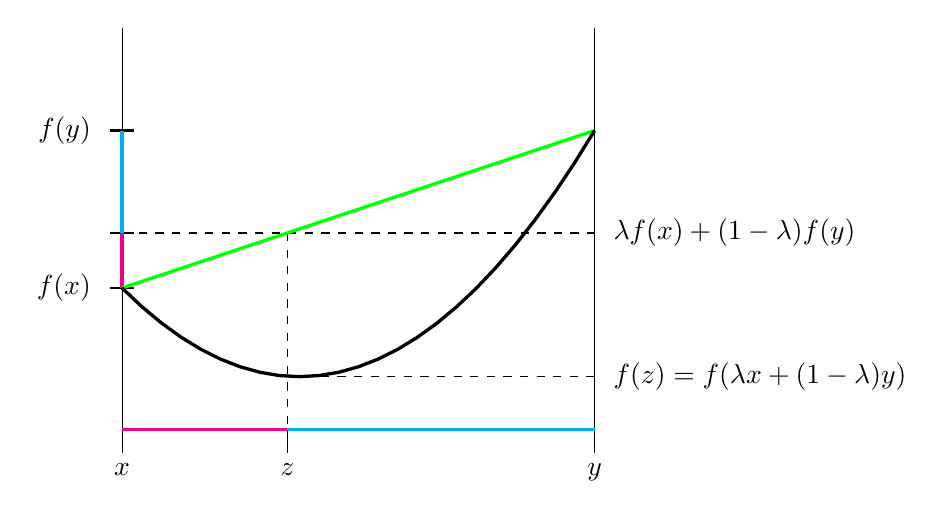
\begin{tikzpicture}[xscale=1.5, yscale = 1.5, scale = 1, declare
      function = { %
        f(\x) = (\x+2)*(\x-1)/3; %
        g(\x) = \x; %
      },] %
      \draw (-2,2.2) -- (-2,-1.4) node[below] {$x$}; %
      \draw (2,2.2) -- (2,-1.4) node[below] {$y$}; %
      \draw (-2,-1.2) -- (2,-1.2); %
      \draw[dashed] (-0.6,7/15) -- (-0.6,-1.2); %
      \draw (-0.6,-1.2) -- (-0.6,-1.4) node[below] {$z$}; %
      \draw[dashed] (-0.6,-0.75) -- (2,-0.75) node[right] {$\
        f(z)=f(\lambda x +(1-\lambda)y)$}; %
      \draw[dashed] (-2,7/15) -- (2,7/15) node[right] %
      {$\ \lambda f(x) + (1-\lambda) f(y)$}; %
      \draw[thick] (-2+0.1,{f(-2)}) -- (-2-0.1,{f(-2)}) node[left]
      {$f(x) \ $}; %
      \draw[thick] (-2+0.1,{f(2)}) -- (-2-0.1,{f(2)}) node[left]
      {$f(y) \ $}; %
      \draw[thick] (-2+0.1,{7/15}) -- (-2-0.1,{7/15}) node[left] {}; %
      %
      \draw[magenta, very thick] (-2,{f(-2)}) -- (-2,{7/15}); %
      \draw[cyan, very thick] (-2,{7/15}) -- (-2,{f(2)}); %
      % 
      \draw[magenta, very thick] (-2, {-1.2}) -- ({-0.6}, -1.2); %
      \draw[cyan, very thick] (-0.6, {-1.2}) -- (2, -1.2); %
      % 
      \draw[green, very thick] (-2, 0) -- (2, 4/3); %
      % 
      \draw[very thick, domain=-2:2] plot (\x, {f(\x)}) node[above]
      {}; %
    \end{tikzpicture}
  \end{center}
  
    
    \begin{remark}
      Cette question est une question de cours. Il faut absolument 
      répondre parfaitement pour mettre le correcteur en confiance.\\ 
      On pouvait aussi utiliser la caractérisation de la convexité 
      avec les tangentes :
      une fonction $f$ est convexe si sa courbe représentative se situe 
      au-dessus de chacune de ses tangentes.
    \end{remark}~\\[-1.4cm]
  \end{proof}
  
  
  

  
  \item Lorsque $f$ est une fonction de classe $\Cont{1}$ sur $[0,1]$, 
  rappeler la caractérisation de la convexité de $f$ sur $[0,1]$ à 
  l'aide de la dérivée $f'$.
  
  \begin{proof}~
    \conc{Si la fonction $f$ est de classe $\Cont{1}$ sur $[0,1]$, 
    alors :\\[.1cm]
    $f$ convexe sur $[0,1]$ 
    \ $\Leftrightarrow$ \ $f'$ 
    croissante sur $[0,1]$.}
    
    \begin{remark}
      Attention à ne pas donner ici la caractérisation pour les 
      fonctions de classe $\Cont{2}$. \\
      Si une fonction $f$ est de classe 
      $\Cont{2}$ sur $[0,1]$, alors :~\\[-.4cm]
      \[
        \text{$f$ convexe sur $[0,1]$} \ \ \Leftrightarrow \ \
        \forall x \in [0,1], \ f''(x) \geq 0
      \]~\\[-.6cm]
      L'énoncé insistait bien sur le fait que la fonction $f$ était 
      seulement de classe $\Cont{1}$. D'ailleurs, dans la suite, on ne
      travaillera qu'avec des fonctions seulement {\bf continues} sur 
      $[0,1]$.
    \end{remark}~\\[-1.4cm]
  \end{proof}

 \end{noliste}
 
 \item 
 \begin{noliste}{a)}
  \setlength{\itemsep}{2mm}
  \item Justifier que $\tilde{f}$ est concave sur $[0,1]$.
  
  \begin{proof}~\\
    Montrons que $\tilde{f}$ est concave sur $[0,1]$, c'est-à-dire
    que $-\tilde{f}$ est convexe sur $[0,1]$.\\
    Soit $(t_1,t_2) \in [0,1]^2$. Soit $\lambda \in [0,1]$.
    \[
      \begin{array}{rcl@{\qquad}>{\it}R{3cm}}
        -\tilde{f}(\lambda \, t_1 +(1-\lambda) t_2) &=& 
        f(\lambda \, t_1 +(1-\lambda)t_2) - (\lambda \, t_1 
	+(1-\lambda)t_2)
	\\[.2cm]
	& \leq & \lambda \, f(t_1) +(1-\lambda)f(t_2) - \lambda \, t_1 
	- (1-\lambda)t_2
	& (car $f$ est convexe sur $[0,1]$)
	\nl
	\nl[-.2cm]
	& = & \lambda(f(t_1)-t_1) + (1-\lambda)(f(t_2)-t_2)
	\\[.4cm]
	&=& \lambda (-\tilde{f})(t_1) + (1-\lambda)(-\tilde{f}(t_2))
      \end{array}
    \]
    
    
    \newpage
    
    
    
    Donc la fonction $-\tilde{f}$ est convexe sur $[0,1]$.
    \conc{La fonction $\tilde{f}$ est concave sur $[0,1]$.}
    
    \begin{remark}
      Attention encore une fois : la fonction $f$ n'est pas supposée 
      ici de classe $\Cont{1}$ sur $[0,1]$. Il n'y a donc pas d'autre
      choix que d'utiliser la définition de la convexité.
    \end{remark}~\\[-1.4cm]
  \end{proof}
  
  \item Montrer que $I(f)= 1-2 \ \dint{0}{1}f(t) \dt$. 
  
  \begin{proof}~
    \begin{noliste}{$\sbullet$}
      \item La fonction $\tilde{f}$ est continue sur $[0,1]$ en tant 
      que somme de fonctions continues sur $[0,1]$.\\
      Donc l'intégrale $I(f)$ est bien définie.
      
      \item On calcule alors :
      \[
      \begin{array}{rcl}
        I(f) &=& 2 \dint{0}{1}(t-f(t) \dt \ = \ 
        2 \, \dint{0}{1} t \dt - 2 \, \dint{0}{1} f(t) \dt
        \ = \ 2\Prim{\dfrac{t^2}{2}}{0}{1} - 2 \, \dint{0}{1} f(t) \dt
        \\[.6cm]
        &=& 2 \times \dfrac{1}{2} - 2 \, \dint{0}{1} f(t) \dt
        \ = \ 1- 2 \, \dint{0}{1} f(t) \dt
      \end{array}
      \]
      \conc{$I(f) = 1-2\, \dint{0}{1} f(t) \dt$}~\\[-1.2cm]
    \end{noliste}
  \end{proof}

  
  \item Représenter dans un même repère orthonormé les fonctions $f$ et 
  $t \mapsto t $ et donner une interprétation géométrique de $I(f)$.
  
  \begin{proof}~\\
    Dans l'ensemble du problème, on notera ${\cal C}_f$ la courbe
    représentative de $f$.\\
    La fonction $t\mapsto t$ correspond en fait à la corde de 
    ${\cal C}_f$ sur $[0,1]$. 
    
    \begin{center}
    %% French babel fout la merde : ne pas oublier shorthandoff
    \shorthandoff{;} 
    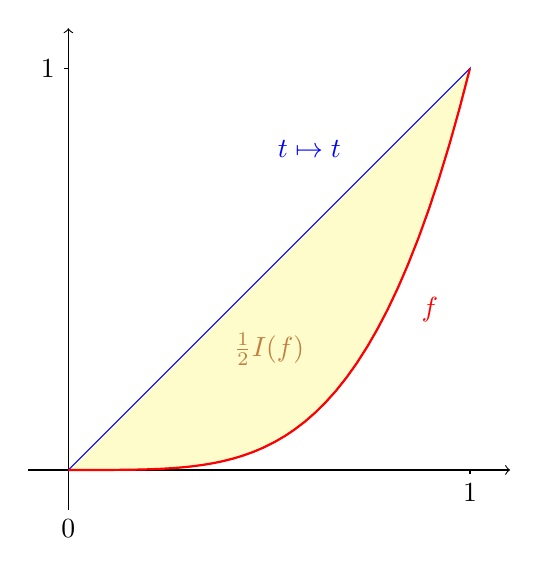
\begin{tikzpicture}[
        xscale = 3, yscale = 3, scale=1.7, %
        declare function = {f(\x) = \x^4;}, %
        declare function = {g(\x) = \x;}, %
        ]
        \draw[->] (-0.1,0) -- (1.1,0); %
        \draw[<-] (0,1.1) -- (0,-0.1) node[below] {$0$}; %
        \draw[-] (0,1) -- (-0.01,1) node[left] {$1$}; %
        \draw[-] (1,0) -- (1,-0.01) node[below] {$1$}; %
        
        \filldraw[draw=blue, fill=yellow!20] %
        (0, 0) -- (0, {f(0)}) plot [domain =0:1] %
        (\x,{f(\x)}) -- (1, 1) -- (0, 0); %
        
        \draw[thick, red, domain=0:1, samples = 40] plot (\x,
        {f(\x)}); %

        \draw[brown] (0.5,0.3) node {$\frac{1}{2} I(f)$};
        \draw[blue] (0.6,0.8) node {$t\mapsto t$};
        \draw[red] (0.9,0.4) node {$f$};
      \end{tikzpicture}
    \end{center}

  On sait que les intégrales $\dint{0}{1} t\dt$ et $\dint{0}{1} 
  f(t)\dt$ mesurent respectivement l'aire sous la courbe de $t \mapsto 
  t$ et l'aire sous la courbe ${\cal C}_f$. 
  \conc{Ainsi, $I(f)$ mesure le double de l'aire entre ${\cal C}_f$ 
   et sa corde sur $[0,1]$.}~\\[-1cm]
  \end{proof}
 \end{noliste}
 
 
 
 \newpage
 
 
 
 \item \textbf{Un premier exemple}.\\
 Soit $f : [0,1] \to \R$ telle que $f(t)= t^2$ pour tout $t \in [0,1]$. 
 \begin{noliste}{a)}
  \setlength{\itemsep}{2mm}
  \item Montrer que $f$ est un élément de $E$.
  
  \begin{proof}~
    \begin{noliste}{$\sbullet$}
      \item La fonction $f$ est bien définie sur $[0,1]$.
      \item De plus : $f(0)=0^2=0$ et $f(1)=1^2=1$.
      \item La fonction $f$ est croissante sur $[0,1]$, donc :
      \[
        \forall t \in [0,1], \ f(0) \leq f(t) \leq f(1)
      \]
      On obtient : $\forall t \in [0,1]$, $0 \leq f(t) \leq 1$.\\
      Donc la fonction $f$ est à valeurs dans $[0,1]$.
      \item La fonction $f$ est bien continue sur $[0,1]$ (en tant 
      que fonction polynomiale).
      \item La fonction $f$ est de classe $\Cont{2}$ sur $[0,1]$ et :
      \[
        \forall t \in [0,1], \ f''(t)=2 \geq 0
      \]
      Donc $f$ est convexe.
    \end{noliste}
    \conc{Finalement : $f\in E$.}~\\[-1cm]
  \end{proof}

  
  \item Calculer $I(f)$. 
  
  \begin{proof}~\\
    D'après la question \itbf{2.b)} :
    \[
      I(f) \ = \ 1-2 \, \dint{0}{1} t^2\dt \ = \ 1- 2 \, 
      \Prim{\dfrac{t^3}{3}}
      {0}{1} \ = \ 1-\dfrac{2}{3} \ = \ \dfrac{1}{3}
    \]
    \conc{$I(f)=\dfrac{1}{3}$}
    
    \begin{remark}
      Ces questions \itbf{3.a)} et \itbf{3.b)} testent la 
      compréhension des notions et notations introduites par l'énoncé.\\
      Ce sont souvent des questions simples qu'il faut repérer et 
      rédiger soigneusement.
    \end{remark}~\\[-1.4cm]
  \end{proof}
 \end{noliste}
 
 \item \textbf{Propriétés de l'indice de Gini.}
 \begin{noliste}{a)}
  \item Pour $f$ élément de $E$, établir que $I(f) \geq 0$. 
  
  \begin{proof}~
    \begin{noliste}{$\sbullet$}
	\item La fonction $f$ est convexe sur $[0,1]$.\\ 
	Sa courbe 
	représentative est donc située en-dessous de sa corde sur 
	$[0,1]$.
	\item Or, la corde sur $[0,1]$ de ${\cal C}_f$ est le segment 
	reliant
	les points $(0,f(0))$ et $(1,f(1))$.\\
	Donc, comme $f\in E$, c'est le segment reliant les points 
	$(0,0)$ et $(1,1)$.\\
	La corde de ${\cal C}_f$ sur $[0,1]$ est la représentation de 
	la fonction
	$t\mapsto t$ sur le segment $[0,1]$.
	
	
	\newpage
	
	
	\item On obtient alors :
	\[
	  \forall t\in [0,1], \ f(t) \leq t \quad \text{donc} \quad 
	  f(t) -t \leq 0
	\]
	Ainsi : $\tilde{f}(t) = t-f(t) \geq 0$.
	\item Par croissance de l'intégrale (les bornes sont dans 
	l'ordre croissant) :
	\[
	  \dint{0}{1} (f(t)-t) \dt \leq 0
	\]
	\conc{D'où :
	$
	  I(f) = 2 \dint{0}{1} \tilde{f}(t) \dt \geq 0
	$.}
      \end{noliste}
    
    \begin{remark}
      Le sujet adopte une approche géométrique de la convexité dès le
      début. On privilégiera donc des réponses de ce type.\\
      On pouvait néanmoins aussi résoudre cette question de la manière 
      suivante.\\
      Soit $t\in [0,1]$.
      \begin{noliste}{$\sbullet$}
	\item On applique l'inégalité de convexité de l'énoncé avec :
	\[
	  t_1=1, \quad t_2=0, \quad \lambda = t
	\]
	On obtient alors :
	\[
	  f(t\times 1 + (1-t) \times 0) \ \leq \ t \, f(1) + (1-t) f(0)
	\]
	Or : $f(0)=0$ et $f(1)=1$. \\
	D'où :
	$
	  f(t) \leq t$. Donc : $\tilde{f}(t)=t-f(t) 
	  \geq 0.
	$
	\item On conclut alors de la même manière que précédemment en 
	utilisant la croissance de l'intégrale.
      \end{noliste}
    \end{remark}~\\[-1.4cm]
  \end{proof}

  
  \item Montrer que $I(f) =0$ si et seulement si $f(t)=t$ pour tout $t 
  \in [0,1]$. 
  
  \begin{proof}~
  \begin{noliste}{$\sbullet$}
    \item Tout d'abord :
    \[
      I(f) = 0 \ \Leftrightarrow \ 2 \dint{0}{1} \tilde{f}(t) \dt =0
      \ \Leftrightarrow \ \dint{0}{1} \tilde{f}(t) \dt=0
    \]

    \item De plus, la fonction $\tilde{f}$ est :
    \begin{noliste}{$\stimes$}
      \item continue sur $[0,1]$, en tant que somme de fonctions
      continues sur $[0,1]$ ;
      \item positive sur $[0,1]$, d'après la question précédente.
    \end{noliste}
    Donc :
    \[
      \dint{0}{1} \tilde{f}(t) \dt = 0 \quad \Leftrightarrow \quad 
      \forall t \in [0,1], \ \tilde{f}(t)=0 \quad 
      \Leftrightarrow \quad \forall t \in [0,1], \ f(t)=t
    \]
  \end{noliste}
  \conc{$I(f)=0$ $\Leftrightarrow$ $\forall t\in [0,1]$, 
  $f(t)=t$}~\\[-1cm]
  \end{proof}
  
  
  
  \newpage
  

  
  \item Montrer que pour tout $f$ élément de $E$, $I(f) < 1$.
  
  \begin{proof}~\\
    Soit $f\in E$.
    \begin{noliste}{$\sbullet$}
      \item D'après la question \itbf{2.b)} :
      \[
        I(f) <1 \ \Leftrightarrow \ 1-2\dint{0}{1} f(t) \dt <1 \
        \Leftrightarrow \ 2 \dint{0}{1} f(t) \dt >0 \ 
        \Leftrightarrow \ \dint{0}{1} f(t) \dt >0
      \]
      
      \item Comme $f$ est à valeurs positives (elle est à valeurs dans 
      $[0,1]$), on a déjà : $\dint{0}{1} f(t) \dt \geq 0$.
      
      \item De plus, la fonction $f$ est :
      \begin{noliste}{$\stimes$}
	\item continue sur $[0,1]$ ;
	\item positive sur $[0,1]$.
      \end{noliste}
      Donc :
      \[
        \dint{0}{1} f(t) \dt = 0 \quad \Leftrightarrow \quad 
        \forall t \in [0,1], \ f(t)=0
      \]
      Cette dernière assertion est fausse car $f(1)=1$.\\
      Donc : $\dint{0}{1} f(t) \dt \neq 0$. D'où : 
      $\dint{0}{1} f(t) \dt >0$
    \end{noliste}
    \conc{Ainsi : $\forall f\in E$, $I(f)<1$.}~\\[-1cm]
  \end{proof}

  
  \item Pour tout entier $n >0$, on définit $f_n$ sur $[0,1]$ par 
  $f_n(t)=t^n$.
  \begin{nonoliste}{(i)}
    \item Pour tout entier $n$ strictement positif, calculer $I(f_n)$.
    
    \begin{proof}~\\
    Soit $n\in \N^*$.
	Commençons par montrer : $f_n \in E$.
	\begin{noliste}{$\sbullet$}
	  \item La fonction $f_n$ est bien définie sur $[0,1]$.
	  \item De plus, comme $n>0$ : $f_n(0)=0^n=0$ et $f_n(1)=1^n=1$.
	  
	  \item La fonction $f_n$ est croissante sur $[0,1]$, donc :
	  \[
	    \forall t\in [0,1], \ f_n(0) \leq f_n(t) \leq f_n(1)
	  \]
	  On obtient : $\forall t\in [0,1]$, $0 \leq f_n(t) \leq 
	  1$.\\
	  Donc la fonction $f_n$ est à valeurs dans $[0,1]$.
	  \item La fonction $f_n$ est bien continue sur $[0,1]$.
	  \item Elle est de classe $\Cont{2}$ sur $[0,1]$ et :
	  \[
	    \forall t \in [0,1], \ f_n''(t)=n(n-1)\geq 0
	  \]
	  Donc $f_n$ est convexe.
	\end{noliste}
	\conc{Finalement : $f_n \in E$.}
	
	
	\newpage
	
	
      D'après la question \itbf{2.b)} :
      \[
        I(f_n) \ = \ 1-2\, \dint{0}{1} t^n \dt \ = \ 1- 2 \, \Prim{
        \dfrac{t^{n+1}}{n+1}}{0}{1} \ = \ 1 - \dfrac{2}{n+1}
      \]
      \conc{$\forall n\in \N^*$, $I(f_n) = 1- \dfrac{2}{n+1}$}
      
      \begin{remark}
        On remarque que l'on retrouve bien le résultat obtenu en 
        question \itbf{3.} pour $n=2$.
      \end{remark}~\\[-1.4cm]
    \end{proof}

    
    \item En déduire que pour tout réel $A$ vérifiant $0 \leq A <1$, il 
    existe $f$ appartenant à $E$ telle que $I(f)>A$. 
    
    \begin{proof}~\\
      Soit $A \in [0,1[$.
	\begin{noliste}{$\sbullet$}
	  \item D'après la question précédente : 
	  $I(f_n)=1-\dfrac{2}{n+1}$.
	  
	  \item Donc :
	  \[
	    \begin{array}{rcl@{\qquad}>{\it}R{5cm}}
	      I(f_n)>A & \Leftrightarrow & 1-\dfrac{2}{n+1}>A
	      \ \Leftrightarrow \ \dfrac{2}{n+1} <1-A
	      \\[.6cm]
	      & \Leftrightarrow & \dfrac{n+1}{2} > \dfrac{1}{1-A}
	      & (par stricte décroissance de $x \mapsto \dfrac{1}{x}$ 
	      sur $]0,+\infty[$)
	      \nl
	      \nl[-.2cm]
	      & \Leftrightarrow & n+1 > \dfrac{2}{1-A} \
	      \Leftrightarrow \ n > \dfrac{2}{1-A}-1
	    \end{array}
	  \]
	  On choisit alors $N=\lceil \dfrac{2}{1-A} -1 \rceil$, et on 
	  obtient : $I(f_N)>A$.
	\end{noliste}
	\conc{Donc pour tout $A\in [0,1[$, il existe $f\in E$ tel que 
	$I(f)>A$.}
	
	\begin{remark}
	  On pouvait aussi se servir de la définition de la limite 
	  d'une suite, comme détaillé ci-dessous.
	  \begin{noliste}{$\sbullet$}
	    \item D'après la question précédente : $\dlim{n\to +\infty}
	    I(f_n)=1$
	    \item Donc, par définition de la limite d'une suite :
	    \[
	      \text{pour tout $A\in [0,1[$, il existe $N\in \N^*$ tel 
	      que $I(f_N)>A$.}
	    \]
	  \end{noliste}
	\end{remark}~\\[-1.4cm]
    \end{proof}

  \end{nonoliste}
 \end{noliste}
 
 \item \textbf{Minoration de l'indice de Gini} 
 \begin{noliste}{a)}
  \item Soit $f$ élément de $E$. Montrer qu'il existe $t_0$ dans 
  $]0,1[$ tel que $\tilde{f}(t_0)= \dmax{t \in [0,1]} \tilde{f}(t)$. 
  
  \begin{proof}~\\
    La fonction $\tilde{f}$ est continue sur le {\bf segment} 
      $[0,1]$.\\
      Elle est donc bornée et atteint ses bornes. En particulier, elle
      est majorée et son maximum est atteint pour un certain réel 
      de $[0,1]$.\\
      Donc il existe $a \in [0,1]$ tel que : $\tilde{f}(a) = 
      \dmax{t\in [0,1]} \tilde{f}(t)$.
      
      
      \newpage
      
      
      Trois cas se présentent alors.
      \begin{noliste}{$\sbullet$}
      \item \dashuline{Si $a \in \ ]0,1[$}. Alors on choisit $t_0=a$.\\
      Et on a effectivement montré qu'il existe $t_0 \in \ ]0,1[$ tel 
      que : $\tilde{f}(t_0) = \dmax{t\in [0,1]}\tilde{f}(t)$.
      
      \item \dashuline{Si $a=0$}. 
      \begin{noliste}{$\stimes$}
      \item Alors :
      \[
        \tilde{f}(a) = \tilde{f}(0) = 0 - f(0)=0
      \]
      
      \item Donc, comme $a$ est un maximum de $\tilde{f}$ sur $[0,1]$,
      on obtient :
      \[
        \forall t\in [0,1], \ \tilde{f}(t) \leq \tilde{f}(a)=0
      \]
      
      \item Or, d'après la question \itbf{4.} : $\forall t\in [0,1]$, 
      $\tilde{f}(t) \geq 0$.\\
      On en déduit : 
      \[
        \forall t \in [0,1], \ \tilde{f}(t) =0 \quad \text{\it (donc 
        $f(t)=t$)}
      \]
      Le maximum de $\tilde{f}$ est donc $0$ et il est atteint en 
      chaque réel du segment $[0,1]$.\\
      On peut donc choisir n'importe quel réel de $]0,1[$ pour $t_0$.\\ 
      Par exemple, on choisit : $t_0=\dfrac{1}{2} \in \ ]0,1[$.
      \end{noliste}
      
      \item \dashuline{Si $a=1$}. Alors, en raisonnant comme pour le 
      cas $a=0$, on obtient :
      \[
        \forall t \in [0,1], \ \tilde{f}(t) =0
      \]
      On choisit donc encore : $t_0=\dfrac{1}{2} \in \ ]0,1[$.
    \end{noliste}
    \conc{Ainsi, il existe toujours $t_0 \in \ ]0,1[$ tel que :
    $\tilde{f}(t_0)=\dmax{t\in [0,1]} \tilde{f}(t)$.}~\\[-1cm]
  \end{proof}

 
  \item Montrer que pour tout $t$ de $[0,t_0]$, $\tilde{f}(t) \geq 
  \tilde{f}(t_0) \cdot \dfrac{t}{t_0}$. 
  
  \begin{proof}~
    \begin{noliste}{$\sbullet$}
      \item La fonction $\tilde{f}$ est concave sur $[0,t_0]$.\\
      Sa courbe représentative est donc située au-dessus de sa corde 
      sur $[0,t_0]$.
      
      \item Or la corde sur $[0,t_0]$ de ${\cal C}_{\tilde{f}}$ est le 
      segment 
      reliant les points $(0,\tilde{f}(0))$ et $(t_0,\tilde{f}(t_0))$.\\
      Donc, c'est le segment reliant 
      $(0,0)$ et $(t_0, \tilde{f}(t_0))$.\\
      Montrons que $y= \tilde{f}(t_0) \cdot \dfrac{t}{t_0}$ est 
      l'équation 
      de la droite $(D)$ passant par ces deux points.
      \begin{noliste}{$\stimes$}
        \item La fonction $t\mapsto \tilde{f}(t_0) \cdot 
	\dfrac{t}{t_0}$ est 
        bien une fonction affine.
        \item Ensuite : $\tilde{f}(t_0) \, \dfrac{0}{t_0} = 0$. \\[.1cm]
        Donc $(D)$ passe bien 
        par le point $(0,0)$.
        \item Enfin : $\tilde{f}(t_0) \, \dfrac{t_0}{t_0} = 
	\tilde{f}(t_0)$. \\[.1cm]
        Donc $(D)$ 
        passe bien par le point $(t_0,\tilde{f}(t_0))$.
      \end{noliste}


%       \begin{noliste}{$\stimes$}
% 	\item Le coefficient directeur de la droite $(D)$ passant par 
% 	ces deux points est :
% 	\[
% 	  \dfrac{f(t_0)-0}{t_0-0} = \dfrac{f(t_0)}{t_0}
% 	\]
% 	Donc l'équation de $(D)$ est de la forme $y=
% 	\dfrac{f(t_0)}{t_0} \,x +b$, avec $b\in \R$.
% 	\item De plus, $(D)$ passe par le point $(0,0)$. Donc :
% 	\[
% 	  0 = \dfrac{f(t_0)}{t_0} \times 0 +b
% 	\]
% 	D'où : $b=0$.
%       \end{noliste}
      La corde de ${\cal C}_{\tilde{f}}$ sur $[0,t_0]$ est donc la 
      représentation 
      de la 
      fonction $t\mapsto \tilde{f}(t_0)\cdot \dfrac{t}{t_0}$
      sur $[0,t_0]$.
    \end{noliste}
    \conc{On en déduit : $\forall t \in [0,t_0]$, $\tilde{f}(t) \geq 
    \tilde{f}(t_0) \, \dfrac{t}{t_0}$}
    
    
    
    
    \newpage
    
    
    
    \begin{remark}
     \begin{noliste}{$\sbullet$}
      \item Comme à la question \itbf{4.a)}, on pouvait
      appliquer 
      l'inégalité de concavité à $\tilde{f}$ avec :
      \[
        t_1 = t_0, \quad t_2 = 0, \quad \lambda = \dfrac{t}{t_0}
      \]
      (on a bien $\lambda \in [0,1]$ car $t\in [0,t_0]$)\\
      On obtient alors :
	\[
	  \tilde{f}\left(\dfrac{t}{\bcancel{t_0}}\times \bcancel{t_0} + 
	  \Big(1- \dfrac{t}{t_0}\Big) \times 0\right) \ \geq \ 
	  \dfrac{t}{t_0} \, \tilde{f}(t_0) + \Big(1-\dfrac{t}{t_0}\Big) 
	  \tilde{f}(0)
	\]
	Or : $\tilde{f}(0)=0$. 
	D'où :
	$
	  \tilde{f}(t) \geq \dfrac{t}{t_0} \tilde{f}(t_0).
	$
      
      \item On peut représenter la situation graphiquement :
      
      \begin{center}
      \scalebox{.95}{$
    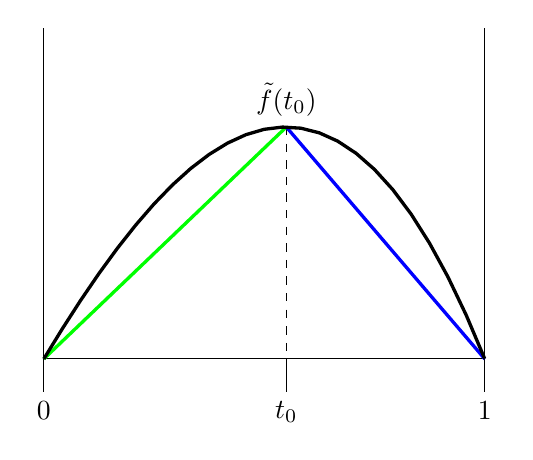
\begin{tikzpicture}[xscale=.8, yscale = 2, scale = 7] %
      \draw (0,.3) -- (0,-0.03) node[below] {$0$}; %
      \draw (1,.3) -- (1,-0.03) node[below] {$1$}; %
      \draw (0,0) -- (1,0) ; %
      \draw[dashed] (0.55,1683/8000) -- (0.55,0); %
      \draw (0.55,0) -- (0.55,-0.03) node[below] {$t_0$}; %
      % 
      \draw[green, very thick] (0, 0) -- (0.55,1683/8000) node[above,
      black] {$\tilde{f}(t_0)$}; %
      \draw[blue, very thick] (0.55, 1683/8000) -- (1, 0) node[right,
      black] {}; %
      %\draw[red, very thick] (-2, 0) -- (2, 4/3); %
      %
      \draw[very thick, domain=0:1] plot (\x, {-\x*(\x+2)*(\x-1)/3})
      node[above] {}; %
    \end{tikzpicture}
    $
    }
    \end{center}~\\[-1cm]
    Le segment vert représente la corde de ${\cal C}_{\tilde{f}}$ sur 
    $[0,t_0]$
    et le segment bleu représente la corde de ${\cal C}_{\tilde{f}}$ 
    sur $[t_0,1]$.
     \end{noliste}
    \end{remark}~\\[-1.4cm]
  \end{proof}

  
  \item Montrer que pour tout $t$ de $[t_0,1]$, $\tilde{f}(t) \geq 
  \tilde{f}(t_0) \cdot \dfrac{t-1}{t_0-1}$. 
  
  \begin{proof}~
    \begin{noliste}{$\sbullet$}
      \item La fonction $\tilde{f}$ est concave $[t_0,1]$.\\
      Sa courbe représentative est donc située au-dessus de sa corde 
      sur $[t_0,1]$.
      
      \item Or la corde sur $[t_0,1]$ de ${\cal C}_{\tilde{f}}$ est le 
      segment 
      reliant les points $(t_0,\tilde{f}(t_0))$ et $(1,\tilde{f}(1))$.\\
      Donc, d'après la question \itbf{5.a)}, c'est le segment reliant 
      $(t_0,\tilde{f}(t_0))$ et $(1,0)$.\\
      Montrons que $y= \tilde{f}(t_0) \cdot \dfrac{t-1}{t_0-1}$ est 
      l'équation de la droite $(d)$ passant par ces deux points.
      \begin{noliste}{$\stimes$}
        \item La fonction $t\mapsto \tilde{f}(t_0) \cdot 
	\dfrac{t-1}{t_0-1}$ est bien une fonction affine.
        \item Ensuite : $\tilde{f}(t_0) \, \dfrac{t_0-1}{t_0-1} = 
        \tilde{f}(t_0)$.\\[.1cm]
        Donc $(d)$ passe bien 
        par le point $(t_0,\tilde{f}(t_0))$.
        \item Enfin : $\tilde{f}(t_0) \, \dfrac{1-1}{t_0-1} = 
	0$.\\[.1cm]
        Donc $(d)$ 
        passe bien par le point $(1,0)$.
      \end{noliste}
%       \begin{noliste}{$\stimes$}
% 	\item Le coefficient directeur de la droite $(D)$ passant par 
% 	ces deux points est :
% 	\[
% 	  \dfrac{1-f(t_0)}{1-t_0} = \dfrac{1-f(t_0)}{1-t_0}
% 	\]
% 	Donc l'équation de $(D)$ est de la forme $y=
% 	\dfrac{1-f(t_0)}{1-t_0} \,x +b$, avec $b\in \R$.
% 	\item De plus, $(D)$ passe par le point $(1,1)$. Donc :
% 	\[
% 	  1 = \dfrac{1-f(t_0)}{1-t_0} \times 1 +b
% 	\]
% 	D'où : 
% 	\[
% 	  b=1- \dfrac{1-f(t_0)}{1-t_0} = \dfrac{\bcancel{1}-t_0 - (
% 	  \bcancel{1}-f(t_0))}{1-t_0} = -\dfrac{f(t_0)-t_0}{t_0-1}
% 	\]
%       \end{noliste}
      La corde de ${\cal C}_{\tilde{f}}$ sur $[t_0,1]$ est donc 
      représentée par la fonction $t \mapsto \tilde{f}(t_0) \cdot
      \dfrac{t-1}{t_0-1}$.
% 
%       
%       
%       
%       \newpage
%       
%       
%       
%       \item Soit $t\in [t_0,1]$. On obtient alors :
%       \[
%         \begin{array}{rcl}
%           f(t) \leq (f(t_0)-1) \, \dfrac{t}{t_0-1} - \dfrac{f(t_0)
%           -t_0}{t_0-1}
%           & \Leftrightarrow & 
%           f(t) -t \leq (f(t_0)-1) \, \dfrac{t}{t_0-1} - \dfrac{f(t_0)
%           -t_0}{t_0-1} -t
%         \end{array}
%       \]
%       Or :
%       \[
%         \begin{array}{rcl}
%           (f(t_0)-1) \, \dfrac{t}{t_0-1} - \dfrac{f(t_0)
%           -t_0}{t_0-1} -t &=& (f(t_0)-1) \, \dfrac{t}{t_0-1} - 
% 	  \dfrac{f(t_0) -t_0}{t_0-1} -\dfrac{(t_0-1)t}{t_0-1}
% 	  \\[.6cm]
% 	  &=& (f(t_0)-\bcancel{1}-(t_0-\bcancel{1}))\dfrac{t}{t_0-1}
% 	  - \dfrac{f(t_0)-t_0}{t_0-1}
% 	  \\[.6cm]
% 	  &=& (f(t_0)-t_0)\dfrac{t}{t_0-1} - \dfrac{f(t_0)-t_0}{t_0-1}
% 	  \\[.6cm]
% 	  &=& (f(t_0)-t_0) \dfrac{t-1}{t_0-1}
%         \end{array}
%       \]
%       On en déduit :
%       \[
%         \begin{array}{rcl}
%           f(t)-t \leq (f(t_0)-t_0) \dfrac{t-1}{t_0-1}
%           & \Leftrightarrow & (t-f(t)) \geq (t_0-f(t_0))
%           \dfrac{t-1}{t_0-1}
%           \\[.6cm]
%           & \Leftrightarrow & \tilde{f}(t) \geq \tilde{f}(t_0)
%           \dfrac{t-1}{t_0-1}
%         \end{array}
%       \]
     \end{noliste}
    \conc{On en déduit : $\forall t \in [t_0,1]$, $\tilde{f}(t) \geq 
    \tilde{f}(t_0) \, \dfrac{t-1}{t_0-1}$}
    
    
    
    
    \newpage
    
    
    
    
    \begin{remark}
      Comme à la question \itbf{4.a)}, on pouvait aussi appliquer 
      l'inégalité de concavité à $\tilde{f}$ avec :
      \[
        t_1 = t_0, \quad t_2 = 1, \quad \lambda = \dfrac{t-1}{t_0-1}
      \]
      (on a bien $\lambda \in [0,1]$ car $t\in [t_0,1]$)
    \end{remark}~\\[-1.4cm]
  \end{proof}
  
  \item En déduire que $I(f) \geq \tilde{f}(t_0)$. 
  
  \begin{proof}~
    \begin{noliste}{$\sbullet$}
      \item D'après la question \itbf{5.b)} :
      \[
        \forall t \in [0,t_0], \ \tilde{f}(t) \geq \tilde{f}(t_0)
        \, \dfrac{t}{t_0}
      \]
      Donc, par croissance de l'intégration (les bornes sont bien
      ordonnées) :
      \[
        \dint{0}{t_0} \tilde{f}(t) \dt \geq \dint{0}{t_0} 
        \tilde{f}(t_0) \, \dfrac{t}{t_0} \dt
      \]
      Or :
      \[
        \dint{0}{t_0} \tilde{f}(t_0) \, \dfrac{t}{t_0} \dt \ = \ 
        \dfrac{\tilde{f}(t_0)}{t_0} \, \dint{0}{t_0} t \dt \ = \
        \dfrac{\tilde{f}(t_0)}{t_0} \, \Prim{\dfrac{t^2}{2}}{0}{t_0} 
        \ = \
        \dfrac{\tilde{f}(t_0)}{2 \, t_0}(t_0^2-0^2) \ = \ 
        \dfrac{\tilde{f}(t_0) \, t_0}{2}
      \]
      \conc{On en déduit :
      $
        \dint{0}{t_0} \tilde{f}(t) \dt \geq \dfrac{\tilde{f}(t_0) \,
        t_0}{2}
      $.}
      
      \item De même, d'après la question \itbf{5.c)} :
      \[
        \forall t \in [t_0,1], \ \tilde{f}(t) \geq \tilde{f}(t_0)
        \, \dfrac{t-1}{t_0-1}
      \]
      Donc, par croissance de l'intégration (les bornes sont bien
      ordonnées) :
      \[
        \dint{t_0}{1} \tilde{f}(t) \dt \geq \dint{t_0}{1}
        \tilde{f}(t_0) \, \dfrac{t-1}{t_0-1} \dt
      \]
      Or :
      \[
       \begin{array}{rcl}
        \dint{t_0}{1} \tilde{f}(t_0) \, \dfrac{t-1}{t_0-1} \dt & = & 
        \dfrac{\tilde{f}(t_0)}{t_0-1} \, \dint{t_0}{1} (t-1) \dt \ = \
        \dfrac{\tilde{f}(t_0)}{t_0-1} \, \Prim{\dfrac{t^2}{2} -t
        }{t_0}{1} 
        \\[.6cm]
        & = &
        \dfrac{\tilde{f}(t_0)}{t_0-1}\left(\dfrac{1^2}{2}-1-\left(
        \dfrac{t_0^2}{2}-t_0\right)\right) \ = \ 
        \dfrac{\tilde{f}(t_0)}{2(t_0-1)}(-t_0^2+2t_0-1)
        \\[.6cm]
        &=& -\dfrac{\tilde{f}(t_0)}{2(t_0-1)}(t_0^2-2t_0+1)
        \ = \ -\dfrac{\tilde{f}(t_0)}{2 \bcancel{(t_0-1)}}
        (t_0-1)^{\bcancel{2}}
        \\[.6cm]
        &=& \dfrac{\tilde{f}(t_0)(1-t_0)}{2}
       \end{array}
      \]
      \conc{On en déduit :
      $
        \dint{t_0}{1} \tilde{f}(t) \dt \geq 
	\dfrac{\tilde{f}(t_0)(1-t_0)}{2}
      $.}
      
      
      
      \newpage
      
      
      
      \item Par relations de Chasles :
      \[
        \begin{array}{rcl}
          I(f) &=& 2 \dint{0}{1} \tilde{f}(t) \dt 
          \\[.6cm]
          &=& 2 \dint{0}{t_0} \tilde{f}(t) \dt + 2 \dint{t_0}{1}
          \tilde{f}(t) \dt 
          \\[.6cm]
          & \geq & \tilde{f}(t_0) \, t_0 + \tilde{f}(t_0) (1-t_0)
          \ = \ \tilde{f}(t_0)
        \end{array}
      \]
      \conc{Ainsi : $I(f) \geq \tilde{f}(t_0)$.}~\\[-1.4cm]
    \end{noliste}
  \end{proof}

 \end{noliste}
 L'indice de Gini donne une indication sur la concentration des 
 richesses d'un pays si l'on suppose que la fonction $f$ rend compte de 
 cette concentration. Par exemple, $f(0,3)=0,09$ s'interprète par le 
 fait que dans la population classée par ordre de richesse croissante, 
 les premiers $30 \%$ de la population possèdent $9\%$ de la richesse 
 totale du pays. Plus l'indice $I(f)$ est grand, plus la répartition 
 des richesses est inégalitaire.
\end{noliste}



\section*{Partie II - Le cas à densité}

\noindent
Soit $g$ une densité de probabilité sur $\R$, nulle sur $]-\infty, 0]$, 
continue et strictement positive sur $]0,+\infty[$. On définit une 
fonction $G$ sur $\R_+$ par $G(x)=\dint{0}{x} g(v) \ dv$ pour $x \in 
\R_+$. Si $g$ représente la densité de population classée suivant son 
revenu croissant, $G(x)$ représente la proportion de la population dont 
le revenu est inférieur à $x$. On suppose de plus que 
$\dint{0}{+\infty} v \, g(v) \ dv$ est convergente et on note $m$ sa 
valeur qui représente donc la richesse moyenne de la population. 

\begin{noliste}{1.}
 \setlength{\itemsep}{4mm}
 \setcounter{enumi}{5}
 \item 
 \begin{noliste}{a)}
  \setlength{\itemsep}{2mm}
  \item Montrer que $m >0$.
  
  \begin{proof}~\\
    La fonction $v \mapsto v \, g(v)$ est :
    \begin{noliste}{$\stimes$}
      \item continue sur $]0,+\infty[$, en tant que produit de fonctions
      continues sur $]0,+\infty[$ ;
      \item {\bf strictement} positive sur $]0,+\infty[$.
    \end{noliste}
    \conc{Donc, par positivité de l'intégrale : $m=
    \dint{0}{+\infty} v \, g(v) \ d v >0$.}~\\[-1cm]
  \end{proof}

  
  \item Montrer que $G$ est une bijection de $[0,+\infty[$ sur $[0,1[$. 
  On notera $G^{-1}$ son application réciproque.
  
  \begin{proof}~
    \begin{noliste}{$\sbullet$}
      \item La fonction $g$ est nulle en dehors de $]0,+\infty[$. Donc,
      pour tout $x\geq 0$ :
      \[
        \dint{-\infty}{x} g(v) \ dv \ = \ \dint{0}{x} g(v) \ dv
        \ = \ G(x)
      \]
      On en déduit que la fonction $G$ coïncide sur $\R_+$ avec la 
      fonction de répartition associée à la densité $g$.\\
      En particulier, la fonction $G$ :
      \begin{noliste}{$\stimes$}
	\item est continue sur $\R_+$,
	\item est croissante sur $\R_+$,
	\item vérifie : $\dlim{x\to +\infty} G(x) =1$.
      \end{noliste}
      
      
      
      \newpage
      
      
      
      \item La fonction $g$ est continue sur $]0,+\infty[$.\\
      Donc, en 
      tant que primitive de $g$, la fonction $G$ est de classe 
      $\Cont{1}$ sur $]0,+\infty[$. \\
      De plus, pour tout $x\in \ ]0,+\infty[$ :
      \[
        G'(x) = g(x) >0
      \]
      D'où $G$ est strictement croissante sur $]0,+\infty[$, donc 
      strictement croissante sur $[0,+\infty[$ (car $g(0)=0$ et donc :
      $\forall x>0$, $g(x) >g(0)$).
      
      \item En résumé, la fonction $G$ est :
      \begin{noliste}{$\stimes$}
	\item continue sur $[0,+\infty[$,
	\item strictement croissante sur $[0,+\infty[$.
      \end{noliste}
      Ainsi, $G$ réalise une bijection de $[0,+\infty[$ sur 
      $G([0,+\infty[)$.
      \[
        G([0,+\infty[) = \left[ G(0), \dlim{x\to +\infty} G(x)\right[
        =[0,1[
      \]
      \conc{La fonction $G$ réalise une bijection de $[0,+\infty[$ sur 
      $[0,1[$.}~\\[-1.2cm]
    \end{noliste}
  \end{proof}

  
  \item Quel est le sens de variation de $G^{-1}$ sur $[0,1[$ ?
  
  \begin{proof}~\\
    D'après le théorème de la bijection, la fonction $G^{-1}$ est 
    continue sur $[0,1[$ et strictement monotone sur $[0,1[$, de 
    même sens de variation que $G$.
    \conc{La fonction $G^{-1}$ est donc strictement croissante 
    sur $[0,1[$.}~\\[-1cm]
  \end{proof}
 \end{noliste}
 
 \item
 \begin{noliste}{a)}
  \setlength{\itemsep}{2mm}
  \item À l'aide du changement de variable $u=G(v)$, établir que pour 
  tout $t \in [0,1[$, 
  \[
   \dint{0}{t} G^{-1}(u) \ du= \dint{0}{G^{-1}(t)} v \, g(v) \ dv
  \]
  
  \begin{proof}~
  \begin{noliste}{$\sbullet$}
  \item La fonction $G^{-1}$ est continue sur $[0,1[$. \\
  Donc, 
  en particulier, pour tout $t\in [0,1[$, $G^{-1}$ est continue
  sur le segment $[0,t]$.
  \conc{Ainsi, pour tout $t \in [0,1[$, l'intégrale 
  $\dint{0}{t} G^{-1}(u) \ du$ est bien définie.}
  
  \item Soit $t\in \ ]0,1[$. Soit $a>0$.\\
    On effectue le changement de variable $\Boxed{u =G(v)}$, 
      où $G$ est de classe $\Cont{1}$ sur 
      $[a,t] \subset \ ]0,+\infty[$ (d'après la question \itbf{6.b)}).
      \[
      \left|
        \begin{array}{P{8cm}}
          $u = G(v)$ (et donc $v = G^{-1}(u)$) \nl
          $\hookrightarrow$ $du = g(v)\ dv$ 
          %\quad et \quad $dt
          %= \dfrac{1}{\ee^{-t}}\ du = \dfrac{1}{1-u} \ du$ 
          \nl
          \vspace{-.4cm}
          \begin{noliste}{$\sbullet$}
          \item $v = G^{-1}(a) \ \Rightarrow \ u = G(G^{-1}(a))=a$
          \item $v = G^{-1}(t) \ \Rightarrow \ u = G(G^{-1}(t))=t$ %
            \vspace{-.4cm}
          \end{noliste}
        \end{array}
      \right.
      \]
      
      
      
      \newpage
      
      
      
      On obtient finalement :
      \[
        \dint{a}{t} G^{-1}(u) \ du \ = \ 
	\dint{G(G^{-1}(a))}{G(G^{-1}(t))}
        G^{-1}(u) \ du \ = \ \dint{G^{-a}}{G^{-1}(t)} G^{-1}(G(v)) \, 
	g(v) \ dv \ = \ \dint{G^{-1}(a)}{G^{-1}(t)} v \, g(v) \ dv
      \]
    Or : $\dlim{a\to 0} G^{-1}(a)=G^{-1}(0)=0$.\\
    De plus, d'après l'énoncé, $\dint{0}{+\infty} v \, g(v) \ dv$ 
    converge en $0$.
    \conc{Donc : $\forall t \in [0,1[$, $\dint{0}{t} G^{-1}(u) \ du
    = \dint{0}{G^{-1}(t)} v \, g(v) \ dv$.}~\\[-1.2cm]
   \end{noliste}
  \end{proof}
  
  \item En déduire que $\dint{0}{1} G^{-1}(u) \ du$ converge et donner 
  sa valeur. 
  
  \begin{proof}~\\
    D'après la question \itbf{6.b)} : $\dlim{t\to 1^-} G^{-1}(t) = 
    +\infty$.\\
    Or l'intégrale $\dint{0}{+\infty} v \, g(v) \ dv$ converge.\\
    D'après la question précédente, on en déduit que l'intégrale
    $\dint{0}{1}
    G^{-1}(u) \ du$ converge et :
    \[
      \dint{0}{1} G^{-1}(u) \ du = \dint{0}{+\infty} v \, g(v) \ dv
      =m
    \]
    \conc{L'intégrale $\dint{0}{1} G^{-1}(u) \ du$ converge et 
    vaut $m$.}~\\[-1cm]
  \end{proof}

 \end{noliste}
 
 \item Soit $f$ la fonction définie sur $[0,1]$ par : $f(t)= 
 \dfrac{1}{m} \dint{0}{t} G^{-1}(u) \ du$ pour tout $t \in [0,1[$ et 
 $f(1)=1$.
 \begin{noliste}{a)}
  \setlength{\itemsep}{2mm}
  \item 
  \begin{nonoliste}{(i)}
   \item Montrer que $f$ est continue sur $[0,1]$. 
   
   \begin{proof}~
     \begin{noliste}{$\sbullet$}
      \item La fonction $G^{-1}$ est continue sur $[0,1[$.\\
      Donc elle admet une primitive $F$ de classe $\Cont{1}$ sur 
      $[0,1[$.\\
      On obtient alors :
      \[
        \forall t \in [0,1[, \ f(t) = \dfrac{1}{m}(F(t)-F(0))
      \]
      Donc la fonction $f$ est de classe $\Cont{1}$ sur $[0,1[$ en 
      tant que transformée affine d'une fonction de classe $\Cont{1}$
      sur $[0,1[$.\\
      En particulier, $f$ est continue sur $[0,1[$.
      
      \item De plus, d'après la question précédente :
      \[
        \dlim{t \to 1^-} f(t) = \dfrac{1}{\bcancel{m}} \times 
        \bcancel{m} = 1 = f(1)
      \]
      Donc $f$ est continue en $1$.
     \end{noliste}
     \conc{Finalement, la fonction $f$ est continue sur 
     $[0,1]$.}~\\[-1cm]
   \end{proof}

   
   
   
   \newpage
   
   
   
   \item Montrer que $f$ est convexe sur $[0,1[$. \textbf{On admettra 
   qu'en fait $f$ est convexe sur $[0,1]$}. 
   
   \begin{proof}~
     \begin{noliste}{$\sbullet$}
      \item D'après la question précédente, la fonction $f$ est de 
      classe $\Cont{1}$ sur $[0,1[$.\\
      De plus, comme $F$ est une primitive de $G^{-1}$, on obtient, 
      pour tout $t\in [0,1[$ :
      \[
        f'(t) = \dfrac{1}{m} \, F'(t) = \dfrac{1}{m} \, G^{-1}(t)
      \]
      
      \item Or, d'après la question \itbf{6.c)}, la fonction $G^{-1}$
      est strictement croissante sur $[0,1[$.\\[.1cm]
      Donc, comme $\dfrac{1}{m} >0$, $f'$ est strictement croissante
      sur $[0,1[$.
      \conc{D'où, d'après la question \itbf{1.b)}, $f$ est 
      convexe sur $[0,1[$.}~\\[-1.2cm]
     \end{noliste}
   \end{proof}
   
   \item En déduire que $f$ est un élément de $E$.
   
   \begin{proof}~
     \begin{noliste}{$\sbullet$}
      \item D'après la question \itbf{8.a)(i)}, la fonction $f$ est 
      continue sur $[0,1]$.
      \item D'après la question \itbf{8.a)(ii)}, la fonction $f$ 
      est convexe sur $[0,1]$.
      \item $f(0)=\dfrac{1}{m} \, \dint{0}{0} G^{-1}(u) \ du =0$
      \item $f(1)=1$
      \item D'après la question précédente : $f'=\dfrac{1}{m} \,
      G^{-1}$.\\[.1cm]
      Or la fonction $G^{-1}$ est à valeurs dans $[0,+\infty[$.\\
      D'où : $\forall t \in [0,1[$, $f'(t) \geq 0$. Ainsi $f$ est 
      croissante sur $[0,1[$, donc sur $[0,1]$ par continuité.\\
      Soit $t\in [0,1]$. On a alors :
      \[
        f(0) \ \leq \ f(t) \ \leq \ f(1)
      \]
      Donc : $0\leq f(t) \leq 1$. Ainsi $f$ est à valeurs dans $[0,1]$.
     \end{noliste}
     \conc{Finalement : $f\in E$.}~\\[-1cm]
   \end{proof}
  \end{nonoliste}
  
  \item Montrer, à l'aide d'une intégration par parties, l'égalité
  \[
   I(f)= -1+\dfrac{2}{m} \dint{0}{\infty} v \, g(v) \, G(v) \ dv
  \]
  
  \begin{proof}~
    \begin{noliste}{$\sbullet$}
      \item Tout d'abord, d'après la question \itbf{2.b)} :
      \[
        I(f) = 1-2 \, \dint{0}{1} f(t) \dt
      \]
      On s'intéresse donc au calcul de l'intégrale 
      $\dint{0}{1} f(t) \dt$.

      \item Soit $a\in [0,1[$. On effectue l'intégration par parties 
      (IPP) suivante.
      \[
	\renewcommand{\arraystretch}{2.2}
	\begin{array}{|rcl@{\qquad}rcl}
	  u(t) & = & f(t) & u'(t) & = & f'(t) \ = \ \dfrac{1}{m} \, 
	  G^{-1}(t) \\
	  v'(t) & = & 1 & v(t) & = & t
	\end{array}
      \]
      
      
      
      \newpage
      
      
      Cette IPP est valide car les fonctions $u$ et $v$ sont de classe 
      $\Cont{1}$ sur $[0,a]$. On obtient :
      \[
        \begin{array}{rcl}
          \dint{0}{a} f(t) \dt &=& \Prim{t \, f(t)}{0}{a} - 
          \dfrac{1}{m} \, \dint{0}{a} t \, G^{-1}(t) \dt
          \\[.6cm]
          &=& a \, f(a) - \dfrac{1}{m} \, \dint{0}{a} t \, G^{-1}(t) \dt
          \quad (*)
        \end{array}
      \]
      On sait déjà : $\dlim{a\to 1^-} a \, f(a) = 1\times f(1)=1$.\\
      On s'intéresse donc au calcul de l'intégrale 
      $\dint{0}{a} t \, G^{-1}(t) \dt$.
      
      \item Comme en question \itbf{7.a)}, on effectue le changement de 
      variable $\Boxed{t =G(v)}$, 
      où $G$ est de classe $\Cont{1}$ sur 
      $[0,1]$.
      \[
      \left|
        \begin{array}{P{8cm}}
          $t = G(v)$ (et donc $v = G^{-1}(t)$) \nl
          $\hookrightarrow$ $dt = g(v)\ dv$ 
          %\quad et \quad $dt
          %= \dfrac{1}{\ee^{-t}}\ du = \dfrac{1}{1-u} \ du$ 
          \nl
          \vspace{-.4cm}
          \begin{noliste}{$\sbullet$}
          \item $v = 0 \ \Rightarrow \ t = G(0)=0$
          \item $v = G^{-1}(a) \ \Rightarrow \ t = G(G^{-1}(a))=a$ %
            \vspace{-.4cm}
          \end{noliste}
        \end{array}
      \right.
      \]
      On obtient finalement :
      \[
       \begin{array}{rcl}
        \dint{0}{a} t \, G^{-1}(t) \dt & = & 
	\dint{0}{G(G^{-1}(a))} t \, 
        G^{-1}(t) \dt
        \\[.6cm]
        & = & \dint{0}{G^{-1}(a)} G(v) \, G^{-1}(G(v)) \, 
	g(v) \ dv
	\\[.6cm]
	& = & \dint{0}{G^{-1}(a)} G(v) \, v \, g(v) \ dv
       \end{array}
      \]
      
      \item On en déduit, avec $(*)$ :
      \[
        \dint{0}{G^{-1}(a)} v \, g(v) \, G(v) \ dv = m \left(
        a f(a) - \dint{0}{a} f(t) \dt \right)
      \]
      Or : $\dlim{a \to 1^-} a \, f(a)=1$. \\
      De plus $\dint{0}{1} 
      f(t) \dt$ converge, car $f$ est continue sur $[0,1]$.\\
      Donc,  
      l'intégrale $\dint{0}{+\infty} v \, g(v) \, G(v) \ dv$ 
      converge (car : $\dlim{a\to 1^-} G^{-1}(a) =+\infty$).
      
      \item On obtient alors :
      \[
        \begin{array}{rcl}
          I(f) &=& 1-2 \dint{0}{1} f(t) \dt
          \\[.6cm]
          &=& 1 - 2 \left(1- \dfrac{1}{m} \dint{0}{+\infty} v \, 
          g(v) \, G(v) \ dv \right)
          \\[.6cm]
          &=& -1 + \dfrac{2}{m} \, \dint{0}{+\infty} v \, g(v) \, 
          G(v) \ dv
        \end{array}
      \]
      \conc{$I(f) = -1 + \dfrac{2}{m} \, \dint{0}{+\infty} v \, 
      g(v) \, G(v) \ dv$}~\\[-1.2cm]
    \end{noliste}
  \end{proof}

 \end{noliste}
 
 
 \newpage
 
 
 \item Soit $\lambda$ un réel strictement positif. On suppose dans 
 cette question que $g$ est une densité de la loi exponentielle de 
 paramètre $\lambda$.
 \begin{noliste}{a)}
  \setlength{\itemsep}{2mm}
  \item Expliciter $G(x)$ pour $x >0$. 
  
  \begin{proof}~\\
    On rappelle que $G$ coïncide sur $\R_+$ avec la fonction de 
    répartition associée à la 
    densité $g$.\\
    La fonction $G$ coïncide donc ici sur $\R_+$ avec la fonction de 
    répartition d'une \var 
    suivant une loi exponentielle de paramètre $\lambda$.
    \conc{$\forall x>0$, $G(x)=1-\ee^{-\lambda \, x}$}~\\[-1cm]
  \end{proof}
  
  \item Expliciter $G^{-1}(u)$ pour $u \in [0,1[$. 
  
  \begin{proof}~\\
    Soit $u\in [0,1[$. Soit $x\in [0,+\infty[$.
    \[
     \begin{array}{rcl@{\qquad}>{\it}R{3cm}}
      G^{-1}(u)=x & \Leftrightarrow & u = G(x) \ \Leftrightarrow \
      u = 1-\ee^{-\lambda \, x} \ \Leftrightarrow \ 
      1-u = \ee^{-\lambda \, x}
      \\[.2cm]
      & \Leftrightarrow & \ln(1-u) = 
      -\lambda \, x \ \Leftrightarrow \ -\dfrac{1}{\lambda} \,
      \ln(1-u) = x
      & (car $\lambda \neq 0$)
     \end{array}
    \]
    \conc{$\forall u \in [0,1[$, $G^{-1}(u) = -\dfrac{1}{\lambda} \,
    \ln(1-u)$}~\\[-1.2cm]
  \end{proof}

  
  \item Donner la valeur de $m$. 
  
  \begin{proof}~\\
    On note $X$ une \var de loi $\Exp{\lambda}$.\\
    On rappelle que $g$ est une densité de $X$. Donc :
    \[
      m = \dint{0}{+\infty} v \, g(v) \ dv = \E(X)
    \]
    \conc{Ainsi : $\E(X)=\dfrac{1}{\lambda}$.}~\\[-1cm]
  \end{proof}

  
  \item Soit $t \in[0,1[$. Montrer que $f(t)= - \dint{0}{t} \ln(1-u) 
  \ du.$
  
  \begin{proof}~\\
    Soit $t \in [0,1[$.\\
    Par définition de $f$ (question \itbf{8.}) :
    \[
      \begin{array}{rcl@{\qquad}>{\it}R{4cm}}
        f(t) &=& \dfrac{1}{m} \, \dint{0}{t} G^{-1}(u) \ du
        \\[.6cm]
        &=& \dfrac{1}{\frac{1}{\lambda}} \, \dint{0}{t} -\dfrac{1}{
        \lambda} \, \ln(1-u) \ du
        & (d'après \itbf{9.b)} et \itbf{9.c)})
        \nl
        \nl[-.2cm]
        &=& - \dint{0}{t} \ln(1-u) \ du 
        & (par linéarité de l'intégrale)
      \end{array}
    \]
    \conc{$\forall t \in [0,1[$, $f(t) = - \dint{0}{t} \ln(1-u) \ 
    du$}~\\[-1cm]
  \end{proof}

  
  
  \newpage
  
  
  \item En déduire que pour tout $t$ élément de $[0,1[$, on a $f(t)= 
  (1-t)\ln(1-t)+t$. 
  
  \begin{proof}~\\
    On note $h:t\mapsto (1-t) \, \ln(1-t)+t$.\\
    Pour montrer que $f$ coïncide avec $h$, vérifions que $h$ est
    l'unique primitive de $t \mapsto -\ln(1-t)$ qui s'annule en $0$.
    \begin{noliste}{$\sbullet$}
      \item $h(0)=(1-0) \, \ln(1-0) +0=0$
      \item La fonction $h$ est dérivable sur l'intervalle $[0,1[$ en 
      tant que somme et produit de fonctions dérivables sur $[0,1[$.\\
      Soit $t\in [0,1[$.
      \[
        h'(t) = -\ln(1-t) -\bcancel{(1-t)} \dfrac{1}{\bcancel{1-t}}
        +1 = -\ln(1-t) -\bcancel{1} + \bcancel{1} = - \ln(1-t)
      \]
    \end{noliste}
    \conc{Ainsi : $f:t \mapsto (1-t) \ln(1-t) +t$.}
    
    \begin{remark}
    \begin{noliste}{$\sbullet$}
      \item Il était également possible (bien que plus long et 
      périlleux) d'effectuer une intégration par parties. Détaillons 
      cette méthode.\\
      Soit $x\in [0,1[$. On effectue l'intégration par parties 
      (IPP) suivante.
      \[
	\renewcommand{\arraystretch}{2.2}
	\begin{array}{|rcl@{\qquad}rcl}
	  u(t) & = & \ln(1-t) & u'(t) & = & -\dfrac{1}{1-t} \\
	  v'(t) & = & -1 & v(t) & = & 1-t
	\end{array}
      \]
      Cette IPP est valide car les fonctions $u$ et $v$ sont de classe 
      $\Cont{1}$ sur $[0,x]$. On obtient :
      \[
        \begin{array}{rcl}
          f(x) &=& \dint{0}{x} - \ln(1-t) \dt 
          \\[.6cm]
          &=& \Prim{(1-t) \ln(1-t)}{0}{x}
          + \dint{0}{x} \bcancel{(1-t)}\dfrac{1}{\bcancel{1-t}} \dt
          \\[.6cm]
          &=& (1-x) \ln(1-x) + \dint{0}{x} 1 \dt
          \ = \ (1-x) \ln(1-x) + \Prim{t}{0}{x}
          \\[.6cm]
          &=& (1-x) \ln(1-x) + x
        \end{array}
      \]
      
      \item On remarque le choix non usuel d'une primitive de 
      $v':t \mapsto -1$.\\
      On choisit ici $v:t \mapsto 1-t$ plutôt que $v:t \mapsto -t$ 
      dans un soucis de simplification des calculs ultérieurs.
    \end{noliste}
    \end{remark}~\\[-1.4cm]
  \end{proof}
  
  
  
  \newpage
  

  
  \item Justifier la convergence de l'intégrale $\dint{0}{1} 
  (1-t)\ln(1-t) \dt$ et la calculer. 
  
  \begin{proof}~
    \begin{noliste}{$\sbullet$}
      \item La fonction $t\mapsto (1-t) \ln(1-t)$ est continue 
      sur $[0,1[$.
      \item Soit $a\in [0,1[$. On effectue l'intégration par parties 
      (IPP) suivante.
      \[
	\renewcommand{\arraystretch}{2.2}
	\begin{array}{|rcl@{\qquad}rcl}
	  u(t) & = & \ln(1-t) & u'(t) & = & - \dfrac{1}{1-t} \\
	  v'(t) & = & 1-t & v(t) & = & -\dfrac{1}{2}(1-t)^2
	\end{array}
      \]
      Cette IPP est valide car les fonctions $u$ et $v$ sont de classe 
      $\Cont{1}$ sur $[0,a]$. On obtient :
      \[
        \begin{array}{rcl}
          \dint{0}{a} (1-t) \ln(1-t) \dt &=& \Prim{-\dfrac{1}{2}
          (1-t)^2 \, \ln(1-t)}{0}{a} - \dfrac{1}{2} \dint{0}{a} 
          (1-t)^{\bcancel{2}} \dfrac{1}{\bcancel{1-t}} \dt
          \\[.6cm]
          &=& - \dfrac{1}{2} (1-a)^2 \ln(1-a) - \dfrac{1}{2} 
          \, \Prim{-\dfrac{1}{2}(1-t)^2}{0}{a}
          \\[.6cm]
          &=& - \dfrac{1}{2}(1-a)^2 \ln(1-a) + \dfrac{1}{4}((1-a)^2
          -1)
        \end{array}
      \]
    
      \item De plus : $\dlim{a \to 1^-} (1-a)^2=0$.
      \item On a aussi : $\dlim{a\to 1^-} (1-a)=0$ et 
      $\dlim{x\to 0} x^2\ln(x)=0$ (par croissances comparées).\\[.1cm]
      D'où : $\dlim{a\to 1^-} (1-a)^2 \ln(1-a)=0$.
    \end{noliste}
    \conc{L'intégrale $\dint{0}{1} (1-t) \ln(1-t) \dt$ converge 
    et vaut $-\dfrac{1}{4}$.}~\\[-1cm]
  \end{proof}
  
  \item En déduire la valeur de $I(f)$.
  
  \begin{proof}~
  \begin{noliste}{$\sbullet$}
    \item Par définition :
    \[
      I(f) \ = \ 2 \dint{0}{1} \tilde{f}(t) \dt \ = \ 2 \dint{0}{1} 
      (t-f(t)) \dt
    \]
    Cette intégrale est bien définie car la fonction $t \mapsto t - f(t)
    $ est continue sur le segment $[0,1]$ (la fonction $f$ est 
    continue sur $[0,1]$).
    
    \item De plus, d'après la question \itbf{9.e)}, pour tout $t \in 
    [0,1[$ :
    \[
      t-f(t) \ = \ \bcancel{t}-\Big((1-t)\ln(1-t) + \bcancel{t}\Big)
      \ = \ -(1-t)\ln(1-t)
    \]
    
    \item On en déduit, avec la question précédente : 
    \[
      I(f) \ = \ -2\dint{0}{1}(1-t) \ln(1-t) \dt \ = \ -2 
      \left(-\dfrac{1}{4} \right) \ = \ \dfrac{1}{2}
    \]
  \end{noliste}
  \conc{$I(f)=\dfrac{1}{2}$}~\\[-1cm]
  \end{proof}
 \end{noliste}
\end{noliste}


\newpage


\section*{Partie III - Application à une population}

\noindent
Une population de $N$ personnes est divisée en deux classes 
(typiquement hommes et femmes) et en $n$ catégories (par exemple 
socio-professionnelles), suivant le tableau à double entrée suivant où 
tous les $x_i$ et $y_i$ pour $i$ dans $\llb 1,n \rrb$ sont des entiers 
naturels. \\
On suppose en outre que pour tout $i$ dans $\llb 1,n \rrb$, 
$x_i \neq 0$. \\ 
\begin{center}
 \begin{tabular}{|c|c|c|c|c|c|c|c|c|}
  \hline
  \backslashbox{Classes}{Catégories} & $c_1$ & $c_2$ & $c_3$ & $\cdots$ 
  & $c_i$ & $\cdots$ & $c_n$ & Total \\ 
  \hline
  I & $x_1$ & $x_2$ & $x_3$ & $\cdots$ & $x_i$ & $\cdots$ & $x_n$ & $X$ 
  \\ 
  \hline
  II & $y_1$ & $y_2$ & $y_3$ & $\cdots$ & $y_i$ & $\cdots$ & $y_n$ & 
  $Y$ \\ 
  \hline
  Total & $n_1$ & $n_2$ & $n_3$ & $\cdots$ & $n_i$ & $\cdots$ & $n_n$ & 
  $N$ \\ 
  \hline
 \end{tabular}
\end{center}

\noindent
où on a donc posé $X= \Sum{i=1}{n} x_i$, $Y= \Sum{i=1}{n} y_i$ et 
$X+Y=N$. On suppose en outre que $Y>0$. \\
Pour $i$ appartenant à $\llb 1,n\rrb$, on adopte les notations 
suivantes: 
\[
 p_i=\dfrac{n_i}{N}, \ q_i=\dfrac{x_i}{X},  \ r_i=\dfrac{y_i}{Y}
\]
On note aussi $\varepsilon_i= \dfrac{x_i}{n_i}$, et 
$\varepsilon=\dfrac{X}{N}$, et on suppose que les catégories sont 
numérotées de telle sorte que : 
\[
 \varepsilon_1 \leq \varepsilon_2 \leq \cdots \leq \varepsilon_n
\]

\begin{noliste}{1.}
 \setlength{\itemsep}{4mm}
 \setcounter{enumi}{9}
 \item On pose $\Omega=\{c_1,c_2, \ldots ,c_n\}$, ensemble des 
 catégories dans la population.
 \begin{noliste}{a)}
  \setlength{\itemsep}{2mm}
  \item Montrer que $P=(p_i)_{1 \leq i \leq n}$, $Q= (q_i)_{1 \leq i 
  \leq n}$ et $R= (r_i)_{1 \leq i \leq n}$ sont des distributions de 
  probabilités.
  
  \begin{proof}~
    \begin{noliste}{$\sbullet$}
      \item Soit $i\in \llb 1,n \rrb$.\\
      D'après l'énoncé : $x_i
      \in \N^*$ et $y_i \in \N$.\\
      Donc : $n_i =x_i+y_i \in \N^*$. En particulier : $n_i > 0$.\\
      De plus : $N=X+Y$, avec $X= \Sum{i=1}{n} x_i > 0$ et $Y>0$.\\
      Donc $N>0$.
      \conc{On en déduit : $\forall i \in \llb 1,n \rrb$, $p_i = 
      \dfrac{n_i}{N} > 0$.}
      
      \item On calcule :
      \[
      \begin{array}{rcl}
        \Sum{i=1}{n} p_i & = & \Sum{i=1}{n} \dfrac{n_i}{N} \ = \ 
        \dfrac{1}{N} \Sum{i=1}{n} n_i \ = \ \dfrac{1}{N} \Sum{i=1}{n}
        (x_i+y_i) 
        \\[.6cm]
        & = & \dfrac{1}{N} \left(\Sum{i=1}{n} x_i + 
	\Sum{i=1}{n} y_i \right) \ = \
        \dfrac{1}{N}(X+Y) \ = \ \dfrac{N}{N} \ = \ 1
      \end{array}
      \]
      \conc{$\Sum{i=1}{n} p_i=1$}
    \end{noliste}
    \conc{Donc $P$ est une loi de probabilité.\\
    De même, $Q$ et $R$ sont des lois de probabilité.}~\\[-1cm]
  \end{proof}
  
  
  \newpage
  

  
  \item Montrer que : $\dfrac{q_1}{p_1} \leq \cdots \leq 
  \dfrac{q_n}{p_n}$ $(\ast)$
  
  \begin{proof}~
  \begin{noliste}{$\sbullet$}
    \item Soit $i \in \llb 1,n \rrb$.
    \[
      \dfrac{q_i}{p_i} \ = \ \dfrac{\frac{x_i}{X}}{\frac{n_i}{N}}
      \ = \ \dfrac{N}{X} \, \dfrac{x_i}{n_i} \ = \ \dfrac{\eps_i}{\eps}
    \]
    \item Or, d'après l'énoncé :
    \[
      \eps_1 \leq \eps_2 \leq \cdots \leq \eps_n
    \]
    \item De plus : $\eps = \dfrac{X}{n} >0$.\\
    En effet, d'après la question précédente : $X>0$ et $N>0$.
    \item On obtient donc :
    \[
      \dfrac{\eps_1}{\eps} \ \leq \ \dfrac{\eps_2}{\eps} \ \leq \ 
      \ldots \ \leq \ \dfrac{\eps_n}{\eps}
    \]
    \end{noliste}
    \conc{Ainsi : $\dfrac{q_1}{p_1} \leq \cdots \leq \dfrac{q_n}{p_n}$
    }~\\[-1cm]
  \end{proof}
  
  \item Montrer que : $\dfrac{r_1}{p_1} \geq \cdots \geq 
  \dfrac{r_n}{p_n}$.
  
  \begin{proof}~
    \begin{noliste}{$\sbullet$}
    \item Soit $i \in \llb 1,n \rrb$.
    \[
      \dfrac{r_i}{p_i} \ = \ \dfrac{\frac{y_i}{Y}}{\frac{n_i}{N}}
      \ = \ \dfrac{N}{Y} \, \dfrac{y_i}{n_i} \ = \ \dfrac{N}{Y} \, 
      \dfrac{n_i-x_i}{n_i} \ = \ \dfrac{N}{Y} (1-\eps_i)
    \]
    \item Or, d'après l'énoncé :
    \[
      \eps_1 \leq \eps_2 \leq \cdots \leq \eps_n
    \]
    Donc :
    \[
      1-\eps_1 \ \geq \ 1-\eps_2 \ \geq \ \cdots \ \geq \ 1-\eps_n
    \]
    \item De plus : $\dfrac{N}{Y} >0$.
    En effet : $N>0$ et $Y>0$.
    \item On obtient donc :
    \[
      \dfrac{N}{Y}(1-\eps_1) \ \geq \ \dfrac{N}{Y}(1-\eps_2) \ \geq \ 
      \ldots \ \geq \ \dfrac{N}{Y}(1-\eps_n)
    \]
    \end{noliste}
    \conc{Ainsi : $\dfrac{r_1}{p_1} \geq \cdots \geq \dfrac{r_n}{p_n}$
    }~\\[-1cm]
  \end{proof}

  
  \item Montrer que pour $i$ appartenant à $\llb 1,n \rrb$, $r_i= 
  \dfrac{n_i-x_i}{N-X}= \dfrac{p_i-\varepsilon q_i}{1- \varepsilon}$. 
  
  \begin{proof}~\\
    Soit $i\in \llb 1,n \rrb$.
    \begin{noliste}{$\sbullet$}
      \item Tout d'abord :
      $r_i \ = \ \dfrac{y_i}{Y} \ = \ \dfrac{n_i-x_i}{N-X}$
      
      \item De plus : 
      \[
        \dfrac{p_i-\eps \, q_i}{1-\eps} \ = \ \dfrac{\frac{n_i}{N}
        - \frac{\bcancel{X}}{N} \, \frac{x_i}{\bcancel{X}}}
        {1-\dfrac{X}{N}} \ = \ \dfrac{\frac{n_i-x_i}{\bcancel{N}}}
        {\frac{N-X}{\bcancel{N}}} \ = \ \dfrac{n_i-x_i}{N-X}
      \]
    \end{noliste}
    \conc{$\forall i \in \llb 1,n \rrb$, $r_i = \dfrac{n_i-x_i}{N-X}
    = \dfrac{p_i - \eps \, q_i}{1-\eps}$}~\\[-1cm]
  \end{proof}
 \end{noliste}
 
 
 
 \newpage
 
 
 
 \item Dans un premier temps, nous allons construire une application 
 appartenant à $E$, qui permet de mesurer les inégalités à l'intérieur 
 de la classe I.\\
 On pose $P_0=Q_0=0$, et pour $i \in \llb 1,n \rrb$, $P_i= \Sum{h=1}{i} 
 p_h$ et $Q_i=\Sum{h=1}{i} q_h$. On définit alors l'application 
 $\varphi$ de $[0,1]$ dans $[0,1]$ telle que, pour tout entier $i \in 
 \llb 0,n \rrb$, $\varphi(P_i)=Q_i$ et pour tout entier $i \in \llb 
 0,n-1 \rrb$, $\varphi$ est affine sur le segment $[P_i, P_{i+1}]$. 
 \begin{noliste}{a)}
  \setlength{\itemsep}{2mm}
  \item On suppose \textbf{dans cette question} $n=3$.\\
  Représenter dans un repère orthonormé $\varphi$ lorsque $P= \left( 
  \frac{1}{2}, \frac{1}{4}, \frac{1}{4} \right)$ et $Q=\left( 
  \frac{1}{3}, \frac{1}{6}, \frac{1}{2}  \right)$. 
  
  \begin{proof}~\\
  D'après l'énoncé :
  \begin{noliste}{$\stimes$}
    \item $p_1=\dfrac{1}{2}$ et $q_1 = \dfrac{1}{3}$. Donc : $(P_1,Q_1)
    =(p_1,q_1) = \left(\dfrac{1}{2}, \dfrac{1}{3}\right)$.
    
    \item $p_2=\dfrac{1}{4}$ et $q_2=\dfrac{1}{6}$. Donc : $(P_2,Q_2)
    =(p_1+p_2,q_1+q_2) = \left(\dfrac{3}{4}, \dfrac{1}{2}\right)$.
    
    \item $p_3=\dfrac{1}{4}$ et $q_3 = \dfrac{1}{2}$. Donc : 
    $(P_3, Q_3) = (p_1+p_2+p_3, q_1+q_2+q_3) = (1,1)$.
  \end{noliste}
  On peut résumer ces informations dans le tableau suivant : %
  
  \begin{center}
  \scalebox{0.9}{
  $
    \begin{tabular}{|>{\centering\small}c||
	      *{4}{>{\centering\arraybackslash\small$}m{7mm}<{$}|
	      }}
    \hline
    \rule[18pt]{0pt}{0pt}
    \cellcolor{gray!20} $i$
    \rule[-15pt]{0pt}{0pt} 
    & \cellcolor{gray!20} 0 & \cellcolor{gray!20} 1 & 
    \cellcolor{gray!20} 2 
    & \cellcolor{gray!20} 3
    \\
    \hline
    \rule[18pt]{0pt}{0pt}
    \cellcolor{gray!20} $P_i$
    \rule[-15pt]{0pt}{0pt} 
    & 0 & \dfrac{1}{2} & \dfrac{3}{4} & 1\\
    \hline
    \rule[18pt]{0pt}{0pt}
    \cellcolor{gray!20} $Q_i$
    \rule[-15pt]{0pt}{0pt} 
    & 0 & \dfrac{1}{3} & \dfrac{1}{2} & 1\\
    \hline
    \end{tabular}
  $
  }
  \end{center}
  Comme la fonction $\varphi$ est affine sur chaque segment $[P_i, 
  P_{i+1}]$, il suffit alors de relier les points précédents par des 
  segments. On obtient la figure suivante :~\\[-.6cm]
    \begin{center}
%     \begin{tikzpicture}[ xscale=1, yscale = 1, scale = 5] %
%       \draw[->] (0,0) -- (1.2,0) node[above right] {$t$}; %
%       \draw[<-] (0,1) -- (0,-0.05) node[below] {$0$}; %
%               
%       \draw[-,blue, very thick] (0,0) -- (0.5,0.33); %
%       \draw[blue] (0,0) node {$\bullet$}; %
%       \draw[blue] (0.5,0.33) node {$\bullet$}; %
% 
%       \draw[-, blue, very thick] (0.5,0.33) -- (0.75,0.5); %
%       \draw[blue] (0.75,0.5) node {$\bullet$}; %
%       
%       \draw[-, blue, very thick] (0.75,0.5) -- (1,1); %
%       \draw[blue] (1,1) node {$\bullet$}; %
%       
%       \draw[blue] (0.9,0.6) node {$\varphi$}; %
%       
%       \foreach \k in {0.2,0.4,0.6,0.8,1}{%
% 	\draw[dashed] (\k,0.01) -- (\k,-0.01) node[below] {\k};
% 	\draw[dashed] (0.01,\k) -- (-0.01,\k) node[left] {\k};
%       }
%     \end{tikzpicture}
    \begin{tikzpicture}
    \begin{axis}[small,xmin=0,ymin=0,axis lines=middle, axis equal, 
    xlabel = $t$]
      \addplot table {
        0 0
        0.5   0.33
        0.75  0.5
        1     1
      } ;
      \draw[blue] (90,60) node {$\varphi$};
    \end{axis}
  \end{tikzpicture}
    \end{center}~\\[-1.6cm]
  \end{proof}

  
  \item Montrer que, dans le plan rapporté à un repère orthonormé, la 
  pente de la droite passant par les points de coordonnées $(P_{i-1}, 
  Q_{i-1})$ et $(P_i, Q_i)$ est $u_i=\frac{q_i}{p_i}$ pour $i$ 
  appartenant à $\llb 1,n \rrb$. 
  
  \begin{proof}~\\
    Soit $i \in \llb 1,n \rrb$.\\
    Le coefficient directeur de la droite passant par $(P_{i-1},
    Q_{i-1})$ et $(P_i,Q_i)$ est donné par :
    \[
      \dfrac{Q_i-Q_{i-1}}{P_i - P_{i-1}} \ = \ \dfrac{\Sum{h=1}{i} q_h 
      - \Sum{h=1}{i-1} q_h}{\Sum{h=1}{i} p_h - \Sum{h=1}{i-1} p_h}
      \ = \ \dfrac{q_i}{p_i}
    \]
    \conc{$\forall i \in \llb 1,n \rrb$, $u_i = 
    \dfrac{q_i}{p_i}$}~\\[-1cm]
  \end{proof}
  
  
  
  \newpage
  

  
  \item Montrer que si $i \in \llb 0,n-1 \rrb$ et $t \in [P_i, 
  P_{i+1}]$, on a $\varphi(t) =u_{i+1} (t-P_i)+Q_i$. 
  
  \begin{proof}~\\
    Soit $i \in \llb 0,n-1 \rrb$.
    \begin{noliste}{$\stimes$}
	\item Le coefficient directeur de la droite représentant 
	$\varphi$ 
	sur $[P_i,P_{i+1}]$ est : $u_{i+1} = 
	\dfrac{q_{i+1}}{p_{i+1}}$.\\
	Donc l'expression de la fonction $\varphi$ est de la forme $t 
	\mapsto u_{i+1} \, t +b$, avec $b\in \R$.
	\item De plus, $\varphi(P_i)=Q_i$. Donc :
	\[
	  Q_i = u_{i+1} \times P_i +b
	\]
	D'où : 
	$
	  b= Q_i - u_{i+1} \, P_i
	$
      \end{noliste}
      
      Donc, pour tout $t\in [P_i, P_{i+1}]$ :
      \[
        \varphi(t) = u_{i+1} \, t +(Q_i-u_{i+1} \, P_i) = 
        u_{i+1}(t-P_i) + Q_i
      \]
      \conc{$\forall i \in \llb 0, n-1 \rrb$, $\forall t \in 
      [P_i, P_{i+1}]$, $\varphi(t) = u_{i+1}(t-P_i) +Q_i$}~\\[-1cm]
  \end{proof}
  
  \item \textbf{En admettant} que les inégalités $(\ast)$ de la 
  question \itbf{10.b)} permettent d'affirmer que $\varphi$ est 
  convexe, justifier que $\varphi$ appartient à $E$. 
  
  \begin{proof}~
    \begin{noliste}{$\sbullet$}
      \item La fonction $\varphi$ est définie sur $[0,1]$ car, comme
      $P$ est une loi de probabilité :
      $\forall i \in \llb 0,n \rrb$, $0 \leq P_i \leq 1$.
      \item La fonction $\varphi$ est à valeurs dans $[0,1]$ car :
      \begin{noliste}{$\stimes$}
      \item comme $Q$ est une loi de probabilité :
      $\forall i \in \llb 0,n \rrb$, $0 \leq Q_i \leq 1$.
      \item la fonction $\varphi$ est de plus affine sur chaque 
      intervalle $[P_i,P_{i+1}]$.\\
      Donc, sur cet intervalle : $0 \leq Q_i \leq \varphi(t) \leq 
      Q_{i+1} \leq 1$.
      \end{noliste}
      \item L'énoncé affirme que $\varphi$ est convexe sur $[0,1]$.
      \item Par construction, $\varphi$ est continue sur $[0,1]$ 
      (elle est même affine par morceaux).
      \item $\varphi(0)=\varphi(P_0)=Q_0=0$.
      \item $\varphi(1)=\varphi(P_n) =Q_n =1$.
    \end{noliste}
    \conc{Ainsi : $\varphi \in E$}~\\[-1cm]
  \end{proof}

  
  \item Pour $i \in \llb 0,n-1 \rrb$, calculer $\dint{P_i}{P_{i+1}} 
  \varphi(t) \dt$. 
  
  \begin{proof}~\\
    Soit $i \in \llb 0, n-1 \rrb$.\\
    D'après la question \itbf{11.c)} : $\forall t \in [P_i, P_{i+1}]$, 
    $\varphi(t) = u_{i+1} (t-P_i) + Q_i$. Donc :
    \[
      \begin{array}{rcl@{\qquad}>{\it}R{5cm}}
        \dint{P_i}{P_{i+1}} \varphi(t) \dt &=& 
        \dint{P_i}{P_{i+1}} (u_{i+1}(t-P_i) + Q_i) \dt
        \\[.6cm]
        &=& u_{i+1} \dint{P_i}{P_{i+1}} (t-P_i) \dt +
        \dint{P_i}{P_{i+1}} Q_i \dt
        & (par linéarité de l'intégrale)
      \end{array}
    \]
    
    
    \newpage
    
    
    
    On obtient alors :
    \[
      \begin{array}{rcl@{\qquad}>{\it}R{5cm}}
	\dint{P_i}{P_{i+1}} \varphi(t) \dt
        &=& u_{i+1} \Prim{\dfrac{(t-P_i)^2}{2}}{P_i}{P_{i+1}} + Q_i
        \, \Prim{t}{P_i}{P_{i+1}}
        \\[.6cm]
        &=& u_{i+1} \dfrac{(P_{i_1}-P_i)^2}{2} + Q_i (P_{i+1}-P_i)
        \\[.4cm]
        &=& \dfrac{Q_{i+1}-Q_i}{\bcancel{P_{i+1}-P_i}} \, 
        \dfrac{(P_{i+1}-P_i)^{\bcancel{2}}}{2} + Q_i(P_{i+1}-P_i)
        & (d'après la question \itbf{11.b)})
        \nl
        \nl[-.2cm]
        &=& \dfrac{1}{2} (Q_{i+1}-Q_i)(P_{i+1}-P_i) + Q_i (P_{i+1}-P_i)
        \\[.4cm]
        &=& \dfrac{1}{2}(P_{i+1}-P_i) (Q_{i+1}-Q_i+2Q_i)
        \\[.4cm]
        &=& \dfrac{1}{2} (P_{i+1}-P_i)(Q_{i+1}+Q_i)
      \end{array}
    \]
    \conc{$\forall i \in \llb 0, n-1 \rrb$, $\dint{P_i}{P_{i+1}}
    \varphi(t) \dt = \dfrac{1}{2}(P_{i+1}-P_i)(Q_{i+1}+Q_i)$}~\\[-1cm]
  \end{proof}
  
  \item Exprimer $I(\varphi)$ sous la forme d'une somme en fonction de 
  $P_0, P_1,...,P_n, Q_0,...Q_n$. 
  
  \begin{proof}~
  \begin{noliste}{$\sbullet$}
    \item D'après la question \itbf{2.b)} :
    \[
        I(\varphi) \ = \ 1-2 \, \dint{0}{1} \varphi(t) \dt 
        \ = \ 1-2 \, \dint{P_0}{P_n} \varphi(t) \dt
    \]
    
    \item De plus, d'après la relation de Chasles :
    \[
      \dint{P_0}{P_n} \varphi(t) \dt \ = \ \Sum{i=0}{n-1} 
        \dint{P_i}{P_{i+1}} \varphi(t) \dt
        \ = \ \dfrac{1}{2} \ \Sum{i=0}{n-1} (P_{i+1}-P_i)(Q_{i+1}+Q_i)
    \]
  \end{noliste}
  \conc{On en déduit : $I(\varphi) = 1-\Sum{i=0}{n-1} 
  (P_{i+1}-P_i)(Q_{i+1}+Q_i)$.}~\\[-1cm]
  \end{proof}
 \end{noliste}
 
 \item Nous allons maintenant étudier l'application correspondante pour 
 la classe II.\\
 On pose $P_0=R_0=0$ et pour $i \in \llb 1,n \rrb$ , $P_i = 
 \Sum{h=1}{i} p_h$ et $R_i=\Sum{h=1}{i} r_h$. De même, on définit pour 
 $i$ élément de $\llb 0,n \rrb$, $\Pi_i=1-P_{n-i}$. On considère 
 l'application $\psi$ de $[0,1]$ dans $[0,1]$ telle que pour tout $i 
 \in \llb 0,n \rrb$, $\psi(P_i)=R_i$ et pour tout entier $i \in \llb 0, 
 n-1 \rrb$, $\psi$ est affine sur le segment $[P_i, P_{i+1}]$. 
 \begin{noliste}{a)}
  \setlength{\itemsep}{2mm}
  \item Montrer que la pente de la droite passant par les points de 
  coordonnées $(P_{i-1}, R_{i-1})$ et $(P_i, R_i)$ est $v_i 
  = \frac{r_i}{p_i}$ pour $i \in \llb 1,n \rrb$. 
  
  \begin{proof}~\\
    Soit $i \in \llb 1,n \rrb$.\\
    Le coefficient directeur de la droite passant par $(P_{i-1},
    R_{i-1})$ et $(P_i,R_i)$ est donné par :
    \[
      \dfrac{R_i-R_{i-1}}{P_i - P_{i-1}} \ = \ \dfrac{\Sum{h=1}{i} r_h 
      - \Sum{h=1}{i-1} r_h}{\Sum{h=1}{i} p_h - \Sum{h=1}{i-1} p_h}
      \ = \ \dfrac{r_i}{p_i}
    \]
    \conc{$\forall i \in \llb 1,n \rrb$, $v_i = 
    \dfrac{r_i}{p_i}$}~\\[-1cm]
  \end{proof}
  
  
  
  \newpage
  

  
  \item On considère l'application $\psi^*$ définie pour tout $t \in 
  [0,1]$, par $\psi^*(t)= 1-\psi(1-t)$. 
  \begin{nonoliste}{(i)}
   \item On suppose \textbf{dans cette question} $n=3$.\\
   Représenter dans un même repère orthonormé les courbes 
   représentatives de $\psi$ et $\psi^*$ lorsque $P= \left( 
   \frac{1}{2}, \frac{1}{4}, \frac{1}{4} \right)$ et $R=\left( 
   \frac{2}{3}, \frac{1}{6}, \frac{1}{6}  \right)$. 
   
   \begin{proof}~\\
   Soit $i\in \llb 0, n \rrb$. Par définition de $\psi^*$ :
   \[
     \psi^*(\Pi_i) = 1-\psi(1-\Pi_i) = 1-\psi(P_{n-i}) = 1-R_{n-i}
   \]
   Détaillons, par exemple, le calcul de $\psi^*(\Pi_2)$.
   \begin{noliste}{$\sbullet$}
     \item Tout d'abord : $\Pi_2 = 1-P_{3-2} = 1-P_1 = 1-\dfrac{1}{2}
     =\dfrac{1}{2}$.
     \item De plus : $\psi^*(\Pi_2) = 1-R_{3-2} = 1-R_1=1-\dfrac{2}{3}
     = \dfrac{1}{3}$.
   \end{noliste}
   On procède ensuite comme en question \itbf{11.a)} et on obtient le 
   tableau et la figure suivants :
   
   \begin{minipage}{0.5\linewidth}
   \[
    \begin{tabular}{|>{\centering\small}c||
	      *{4}{>{\centering\arraybackslash\small$}m{7mm}<{$}|
	      }}
    \hline
    \rule[18pt]{0pt}{0pt}
    \cellcolor{gray!20} $i$
    \rule[-15pt]{0pt}{0pt} 
    & \cellcolor{gray!20} 0 & \cellcolor{gray!20} 1 & 
    \cellcolor{gray!20} 2 
    & \cellcolor{gray!20} 3
    \\
    \hline
    \rule[18pt]{0pt}{0pt}
    \cellcolor{gray!20} $P_i$
    \rule[-15pt]{0pt}{0pt} 
    & 0 & \dfrac{1}{2} & \dfrac{3}{4} & 1\\
    \hline
    \rule[18pt]{0pt}{0pt}
    \cellcolor{gray!20} $R_i$
    \rule[-15pt]{0pt}{0pt} 
    & 0 & \dfrac{2}{3} & \dfrac{5}{6} & 1\\
    \hline
    \rule[18pt]{0pt}{0pt}
    \cellcolor{gray!20} $\Pi_i$
    \rule[-15pt]{0pt}{0pt} 
    & 0 & \dfrac{1}{4} & \dfrac{1}{2} & 1\\
    \hline
    \end{tabular}
  \]
  \end{minipage}
  \begin{minipage}{0.5\linewidth}
     \begin{center}
     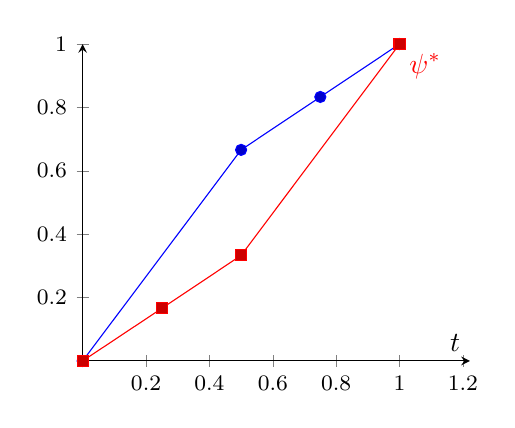
\begin{tikzpicture}
    \begin{axis}[small,xmin=0,ymin=0,axis lines=middle, axis equal, 
      xlabel=$t$]
      \addplot table {
        0 0
        0.5   0.666
        0.75  0.833
        1     1
      };
      \draw[blue] (45, 75) node {$\psi$};
      \addplot table {
        0 0
        0.25   0.166
        0.5  0.333
        1     1
      } node[below right] {$\psi^*$};
    \end{axis}
  \end{tikzpicture}
  \end{center}
  \end{minipage}
   \end{proof}
   
   \item Montrer que $\psi^*$ est convexe sur $[0,1]$. 
   
   \begin{proof}~
     \begin{noliste}{$\sbullet$}
      \item Comme en question \itbf{11.d)}, on admet que les inégalités 
      de \itbf{10.c)} permettent d'affirmer que $\psi$ est concave 
      sur $[0,1]$.
      
      \item Montrons que $\psi^*$ est alors convexe sur $[0,1]$.\\
      Soit $(t_1,t_2) \in [0,1]^2$. Soit $\lambda \in [0,1]$.
      \[
        \begin{array}{rcl@{\qquad}>{\it}R{5cm}}
          \lambda \, \psi^*( t_1) + (1-\lambda) \psi^*(t_2)
          &=& 
          \lambda(1-\psi(1-t_1)) + (1-\lambda) (1-\psi(1-t_2))
          \\[.2cm]
          &=& \bcancel{\lambda} -\lambda \, \psi(1-t_1) + 1 -
          \bcancel{\lambda} + (1-\lambda) \psi(1-t_2)
          \\[.2cm]
          &=& 1- \Big(\lambda \, \psi(1-t_1) + (1-\lambda)\psi(1-t_2)
          \Big)
        \end{array}
      \]
      
      \item Or $(t_1,t_2)\in [0,1]^2$, donc $(1-t_1,1-t_2) \in 
      [0,1]^2$.\\
      D'où, par concavité de $\psi$ :
      \[
        \lambda \, \psi(1-t_1) + (1-\lambda) \psi(1-t_2) \ \leq \ 
        \psi(\lambda \, (1-t_1) + (1-\lambda) t_2)
      \]
      De plus :
      \[
        \psi(\lambda \, (1-t_1) + (1-\lambda)(1-t_2)) \ = \
        \psi(\bcancel{\lambda} - \lambda \, t_1 + 1 - 
        \bcancel{\lambda} - (1-\lambda) t_2) \ = \
        \psi\Big(1-(\lambda \, t_1 + (1-\lambda) t_2) \Big)
      \]
      
      \item On obtient alors :
      \[
        \lambda \, \psi^*( t_1) + (1-\lambda) \psi^*(t_2) \ \geq \
        1-\psi\Big(1-(\lambda \, t_1 + (1-\lambda) t_2) \Big)
      \]
      D'où, par définition de $\psi^*$ :
      \[
        \psi^*(\lambda \, t_1 + (1-\lambda) t_2)
        \ \leq \
        \lambda \, \psi^*( t_1) + (1-\lambda) \psi^*(t_2)
      \]
      \conc{Ainsi, $\psi^*$ est convexe sur $[0,1]$.}~\\[-1.2cm]
     \end{noliste}
   \end{proof}

   
   \item Montrer que $\psi^*$ est affine sur $[\Pi_{i-1}, \Pi_i]$ pour 
   $i \in \llb 0,n-1 \rrb$. 
   
   \begin{proof}~\\
     On note $\sigma$ la fonction $t\mapsto 1 - t$.\\
     Par définition de $\psi^*$ : 
     \[
      \psi^* = \sigma \circ \psi \circ \sigma
     \]
     Or : 
     \begin{noliste}{$\stimes$}
     \item la fonction $\sigma$ est une bijection affine de 
      $[\Pi_{i-1},\Pi_i]$ sur $[P_{n-i},P_{n-i+1}]$, 
     \item la fonction $\psi$ est affine sur $[P_{n-i}, P_{n-i+1}]$. 
     \end{noliste}
     Ainsi, sur $[\Pi_{i-1},\Pi_i]$, la fonction $\psi^*$ est une 
     composition de trois fonctions affines.
     \conc{Donc $\psi^*$ est affine sur $[\Pi_{i-1}, \Pi_i]$.}~\\[-1cm]
   \end{proof}

   
   \item Montrer que la pente de $\psi^*$ sur $[\Pi_{i-1}, \Pi_i]$ est 
   $v_{n-i+1}$ pour $i \in \llb 1,n \rrb$. 
   
   \begin{proof}~\\
     Soit $i \in \llb 1,n \rrb$.\\
    D'après la question \itbf{12.b)(i)}, le coefficient directeur de 
    $\psi^*$ sur $[\Pi_{i-1},
    \Pi_i]$ est donné par :
    \[
      \dfrac{\psi^*(\Pi_i)-\psi^*(\Pi_{i-1})}{\Pi_i - \Pi_{i-1}} \ = \ 
      \dfrac{\bcancel{1}-R_{n-i}-(\bcancel{1}-R_{n-(i-1)})}
      {\bcancel{1}-P_{n-i}-(\bcancel{1}-P_{n-(i-1)})} \ = \
      \dfrac{R_{n-i+1}-R_{n-i}}{P_{n-i+1}-P_{n-i}}
      \ = \ \dfrac{r_{n-i+1}}{p_{n-i+1}} \ = \ v_{n-i+1}
    \]
    \conc{Pour tout $i \in \llb 1,n \rrb$, la pente de 
    $\psi^*$ sur $[\Pi_{i-1}, \Pi]$ est donc $v_{n-i+1}$.}~\\[-1cm]
   \end{proof}
  \end{nonoliste}

  \noindent
  On dit dans cette situation que les fonctions $\varphi$ et $\psi^*$ 
  sont \textbf{adjointes} l'une de l'autre. C'est leur comparaison que 
  Gini a proposé de considérer pour \og mesurer les inégalités \fg{} 
  entre la population de catégorie I et celle de catégorie II. \\
  Une égalité entre les fonctions adjointes signale notamment l'absence 
  totale d'inégalité sociale. La dernière question précise quelque peu 
  ce point. 
 \end{noliste}
 
 \item 
 \begin{noliste}{a)}
  \setlength{\itemsep}{2mm}
  \item Montrer que si $\varphi= \psi^*$ alors pour tout $i$ 
  appartenant à $\llb 1,n \rrb$ :
  \[
   \dfrac{\varepsilon_i}{\varepsilon} = 
   \dfrac{1-\varepsilon_{n-i+1}}{1-\varepsilon}
  \]
  
  \begin{proof}~
    \begin{noliste}{$\sbullet$}
      \item Si $\varphi=\psi^*$, alors ces fonctions sont égales en 
      tout point. En particulier :
      \begin{noliste}{$\stimes$}
	\item pour tout $i \in \llb 0, n \rrb$, $P_i= \Pi_i$ ;
	\item pour tout $i \in \llb 0, n-1 \rrb$, sur chaque 
	intervalle $[P_i,P_{i+1}]$, ${\cal C}_\varphi$ et 
	${\cal C}_{\psi^*}$ ont même pente.
      \end{noliste}
      
      
      \newpage
      
      
      Donc, d'après les questions \itbf{11.b)} et \itbf{12.b)(iv)} :
      \[
        \forall i \in \llb 1, n \rrb, \ u_i = v_{n-i+1}
      \]
      
      \item De plus, d'après les questions \itbf{11.b)} et \itbf{10.b)} 
      :
      \[
        \forall i \in \llb 1, n \rrb, \ u_i= \dfrac{q_i}{p_i}
        = \dfrac{\eps_i}{\eps}
      \]
      
      \item Enfin, d'après les questions \itbf{12.b)(iv)} et 
      \itbf{10.c)} :
      \[
        \forall i \in \llb 1, n \rrb, \ v_{n-i+1}= 
        \dfrac{r_{n-i+1}}{p_{n-i+1}}
        = \dfrac{1-\eps_{n-i+1}}{1-\eps}
      \]
    \end{noliste}
    \conc{Ainsi, si $\varphi = \psi^*$, alors : $\forall i \in \llb 
    1,n \rrb$, $\dfrac{\eps_i}{\eps} = \dfrac{1-\eps_{n-i+1}}{1-\eps}
    $.}~\\[-1cm]
  \end{proof}
  
  \item Montrer que si $\varphi= \psi^*$, alors pour tout $i$ 
  appartenant à $\llb 1,n \rrb$, $\varepsilon_i+ \varepsilon_{n-i+1}=2 
  \varepsilon$. 
  
  \begin{proof}~\\
    Supposons $\varphi=\psi^*$. Soit $i\in \llb 1,n \rrb$.
    \begin{noliste}{$\sbullet$}
      \item D'après la question précédente : $\dfrac{\eps_i}{\eps}
      = \dfrac{1-\eps_{n-i+1}}{1-\eps} \quad (1)$.
      \item On applique cette égalité à $i=n-i+1 \in \llb 1,n \rrb$. 
      On obtient alors :
      \[
        \dfrac{\eps_{n-i+1}}{\eps} = \dfrac{1-\eps_{\bcancel{n}
        -(\bcancel{n}-i+\bcancel{1})+\bcancel{1}}}
        {1-\eps} = \dfrac{1-\eps_i}{1-\eps} \quad (2)
      \]
      
      \item En sommant $(1)$ et $(2)$, on en déduit :
      \[
        \dfrac{\eps_i}{\eps} + \dfrac{\eps_{n-i+1}}{\eps} = 
        \dfrac{1-\eps_{n-i+1}}{1-\eps} + \dfrac{1-\eps_i}{1-\eps}
      \]
      Donc :
      $
        (1-\eps)(\eps_i+\eps_{n-i+1}) = \eps(1-\eps_i +1-\eps_{n-i+1})
        = \eps (2-\eps_i-\eps_{n-i+1}).
      $\\[.1cm]
      D'où :
      $
        (1-\eps)(\eps_i + \eps_{n-i+1}) = 2\eps -\eps(\eps_i + 
        \eps_{n-i+1}).
      $\\[.1cm]
      Ainsi :
      $
        (1-\bcancel{\eps}-(-\bcancel{\eps}))(\eps_i + \eps_{n-i+1}) = 
	2\eps.
      $
    \end{noliste}
    \conc{Si $\varphi = \psi^*$, alors : $\forall i \in \llb 1,n \rrb$,
    $\eps_i + \eps_{n-i+1}=2\eps$.}~\\[-1.4cm]
  \end{proof}

  
  \item Déduire que si $\varphi= \psi^*$, on a pour tout $i$ 
  appartenant à $\llb 1,n \rrb$, $\varepsilon_i(1-2\varepsilon)= 
  \varepsilon(1-2\varepsilon)$.
  
  \begin{proof}~\\
  Supposons $\varphi=\psi^*$. Soit $i \in \llb 1,n \rrb$.
    \begin{noliste}{$\sbullet$}
      \item D'après \itbf{13.b)} : $\eps_i + \eps_{n-i+1}=2\eps$.
      Donc : $\eps_{n-i+1}=2\eps -\eps_i$.
      \item D'après \itbf{13.a)} : $\dfrac{\eps_i}{\eps} = 
      \dfrac{1-\eps_{n-i+1}}{1-\eps}$.
      Donc : $(1-\eps)\eps_i = \eps(1-\eps_{n-i+1})$.
    \end{noliste}
    On obtient donc :
    \[
      (1-\eps)\eps_i=\eps(1-(2\eps-\eps_i)) = \eps(1-2\eps) + \eps \,
      \eps_i
    \]
    D'où :
    \[
      (1-\eps)\eps_i - \eps \, \eps_i = \eps(1-2\eps)
    \]
    \conc{Ainsi, si $\varphi = \psi^*$, alors : $\forall i \in \llb 1,n 
    \rrb$, $\eps_i(1-2\eps) = \eps(1-2\eps)$.}~\\[-1.3cm]
  \end{proof}
  
  
  \newpage

  
  \item On suppose que $\varepsilon \neq \dfrac{1}{2}$.  Montrer que si 
  $\varphi= \psi^*$, alors pour tout $i$ appartenant à $\llb 1,n \rrb$, 
  $\varepsilon_i=\varepsilon$. \\[.1cm]
  Interpréter ce résultat.
  
  \begin{proof}~\\
  Supposons $\varphi=\psi^*$.
    \begin{noliste}{$\sbullet$}
      \item Soit $i \in \llb 1,n \rrb$.\\
      D'après la question précédente : $\eps_i(1-2\eps) = 
      \eps(1-2\eps)$.\\
      Or $\eps \neq \dfrac{1}{2}$, donc $1-2\eps \neq 0$. D'où :
      $
        \eps_i = \eps
      $
      \conc{Si $\varphi = \psi^*$, alors : $\forall i \in \llb 1,n 
      \rrb$, $\eps_i=\eps$.}
      
      \item Lorsque $\varphi = \psi^*$, chaque catégorie présente 
      le même coefficient $\varepsilon_i = \varepsilon$, c'est-à-dire 
      la même proportion $\dfrac{x_i}{n_i} = \varepsilon$ et \emph{a 
      fortiori} la même proportion $\dfrac{y_i}{n_i} = 
      1-\varepsilon$.\\[.1cm]      
      Donc le pourcentage de femmes (ou plus généralement de personnes
      de classe I) est le même dans toutes les catégories 
      socio-professionnelles. 
      \conc{Autrement dit, on n'observe aucune inégalité sociale entre 
      la classe I (les femmes) \\[.1cm]
      et la classe II (les hommes).}~\\[-1cm]
    \end{noliste}
  \end{proof}

 \end{noliste}
\end{noliste}






